%=====================================================================
% When Index Tuning Advice Backfires
% Journal version. Target: Data and Knowledge Engineering / Information Systems
% Class: elsarticle (Elsevier). Compile: pdflatex -> bibtex -> pdflatex x2
%=====================================================================
\documentclass[preprint,12pt,authoryear]{elsarticle}

\usepackage[T1]{fontenc}
\usepackage{graphicx}
\usepackage{booktabs}
\usepackage{amsmath,amssymb}
\usepackage{array}
\usepackage{multirow}
\usepackage{listings}
\usepackage{xcolor}
\usepackage{url}
\usepackage{hyperref}

\journal{Information Systems}

\definecolor{codegray}{gray}{0.96}
\lstdefinestyle{plainstyle}{
    backgroundcolor=\color{codegray},
    basicstyle=\ttfamily\footnotesize,
    numbers=none, frame=single, framerule=0pt,
    breaklines=true, showstringspaces=false, captionpos=b
}
\lstset{style=plainstyle}

\newcommand{\rpc}{\texttt{random\_page\_cost}}
\newcommand{\sbuf}{\texttt{shared\_buffers}}

\begin{document}

\begin{frontmatter}

\title{When Index Tuning Advice Backfires: An Experimental Study of
Access-Path Selection in PostgreSQL}

\author[aiub]{Md. Imtiaj Alam Sajin\corref{cor1}}
\ead{26-94090-2@student.aiub.edu}

\author[aiub]{Ashraf Uddin}
\ead{dr.ashraf@aiub.edu}

\cortext[cor1]{Corresponding author.}

\address[aiub]{Department of Computer Science, American International
University-Bangladesh, 408/1 Kuratoli, Khilkhet, Dhaka 1229, Bangladesh}

\begin{abstract}
Choosing the wrong index can slow a query by orders of magnitude, and a
large body of practitioner guidance exists to prevent that. We ask
whether the guidance survives measurement. We build a benchmark in
which value skew, predicate correlation and physical clustering vary
independently, with ground-truth cardinality computed from the
generated data rather than obtained from the system under test, and
report 18{,}440 query executions against PostgreSQL~17.1 and
MariaDB~10.4 across seven table scales.

Our first result is reassuring: under a conventional index set
PostgreSQL selects a near-optimal access path, erring materially for
2.3\% of queries. Our remaining results are not. Three widely
recommended practices each degrade performance. Extended statistics,
the documented remedy for correlated predicates, improve estimates by
up to 108$\times$ while making queries up to 2.7$\times$ slower, because
the correction is not propagated to the \texttt{BitmapAnd} node that
consumes it. Reducing \rpc{} on flash storage slows the workload by
2.3$\times$, the default lying within 6\% of optimal. Adding a BRIN
index beside a B-tree raises misselection to 73.3\%, with queries
degrading by up to 194$\times$; we trace this to a deduplication step in
\texttt{choose\_bitmap\_and()} that breaks ties on index-side cost
alone, a metric on which BRIN wins by construction while the whole cost
difference lies on the heap side.

Cardinality misestimation does not explain the misselection we observe:
98.2\% of misselected queries had accurate row estimates. Measuring a
second system separates the general from the implementation-specific.
Near-optimal selection is specific, MariaDB misselecting for 66.0\% of
the same queries; the correlated-predicate failure is general,
appearing in MariaDB's \texttt{index\_merge} exactly as in PostgreSQL's
\texttt{BitmapAnd}. The two systems also degrade in opposite directions
as tables grow, one erring more often but never severely, the other
less often but without bound. All code and measurements are published.
\end{abstract}

\begin{keyword}
query optimisation \sep access path selection \sep index selection \sep
cardinality estimation \sep cost model \sep PostgreSQL \sep
performance benchmarking
\end{keyword}

\end{frontmatter}

%=====================================================================
\section{Introduction}
\label{sec:intro}
%=====================================================================

The access-path decision, whether to read a table sequentially or
through one of several available indexes, is among the most
consequential choices a query optimiser makes. It was formalised in the
System~R optimiser \citep{selinger1979access} and the same framework,
estimate cardinality and then price each candidate path, underpins
PostgreSQL today. Depending on that single decision, the same query can
differ by two orders of magnitude in execution time.

Because the decision matters and is opaque to the user, a large body of
tuning guidance has accumulated around it. Administrators are advised to
create extended statistics when predicate columns are correlated
\citep{pgdocs17createstats}, to lower \rpc{} when running on
solid-state storage \citep{pgdocs17runtimeconfig}, and to add
Block Range Index (BRIN) structures on naturally ordered columns
because they are small and inexpensive to build \citep{pgdocs17brin}.
This guidance appears in official documentation, vendor engineering
material and community forums. It is generally justified by a mechanism
argument, an explanation of why the change should help, rather than by
workload-level measurement.

Mechanism arguments are seductive because they are usually correct as
far as they go. Extended statistics really do improve cardinality
estimates. Random reads on flash storage really are cheaper relative to
sequential reads than they were on magnetic disks
\citep{graefe2009fast,lee2009advances}. BRIN indexes really are orders
of magnitude smaller than B-trees. The question this paper asks is
whether being correct about the named quantity is sufficient to improve
the outcome that actually matters, namely the runtime of the workload.

\subsection{Research questions}

\begin{description}
\item[RQ1] How often does the PostgreSQL planner select a slower access
  path than one available to it, and what does that cost?
\item[RQ2] Which data properties drive misselection: value skew,
  correlation between predicate columns, or physical clustering?
\item[RQ3] Is cardinality misestimation the cause, as the query
  optimisation literature would predict?
\item[RQ4] Do the three tuning practices named above improve
  access-path selection?
\item[RQ5] Under what conditions do the observed effects cease to hold?
\item[RQ6] Which of the observed effects are properties of cost-based
  access-path selection in general, and which are artefacts of one
  implementation?
\end{description}

RQ5 deserves emphasis. Empirical database studies frequently report
that an effect exists without establishing the conditions under which
it disappears. That omission is consequential: a practitioner cannot
tell whether a published finding applies to their deployment, and a
subsequent study measuring at a different scale may appear to
contradict the original when in fact both are correct within their
respective regimes. We show in Section~\ref{sec:boundary} that this is
not hypothetical, and that our own two-point comparison would have
yielded a conclusion the intermediate measurements refute.

\subsection{Contributions}

\begin{enumerate}
\item A controlled benchmark in which skew, predicate correlation and
  physical clustering vary independently, with exact ground-truth
  cardinality for every predicate, obtained by counting the generated
  data rather than by querying the system under test.
\item A quantification of PostgreSQL~17's access-path selection
  quality, which we find to be near optimal under a conventional index
  set (Section~\ref{sec:baseline}).
\item Evidence that cardinality misestimation does not explain
  single-table access-path misselection, in contrast to the established
  result for join ordering \citep{leis2015good}
  (Section~\ref{sec:notest}).
\item Three measured cases in which recommended tuning practice
  degrades performance, each traced to a mechanism visible in the query
  plan (Sections~\ref{sec:extstats}--\ref{sec:brin}).
\item A characterisation of the scale boundaries of the largest effect,
  showing that its frequency and its severity collapse at two different
  and separately identifiable system boundaries
  (Section~\ref{sec:boundary}).
\item A fully reproducible artifact: seeded data generation, resumable
  measurement, and one-command regeneration of every figure
  \citep{artifact2026}.
\end{enumerate}

%=====================================================================
\section{Background}
\label{sec:background}
%=====================================================================

\subsection{Access-path selection}

Given a predicate over a single relation, a cost-based optimiser
enumerates candidate access paths, a sequential scan plus one path per
usable index, estimates the number of rows each will produce, and
assigns each a cost \citep{selinger1979access,chaudhuri1998overview,graefe1993query}.
In PostgreSQL, cost is expressed in abstract units anchored to
\texttt{seq\_page\_cost}, with \rpc{} expressing how much more expensive
a randomly fetched page is assumed to be relative to a sequentially
fetched one \citep{pgdocs17indexcost}. The default ratio of 4:1 encodes
an assumption about magnetic disk behaviour.

A bitmap scan occupies an intermediate position between an index scan
and a sequential scan. The index is scanned to build a bitmap of
matching tuple identifiers or block ranges, the bitmap is sorted into
physical order, and the heap is then read in that order, converting
random access into something closer to sequential access. The cost of a
bitmap heap scan is therefore dominated by the number of heap pages the
optimiser expects to fetch, priced using \rpc{} interpolated toward
\texttt{seq\_page\_cost} as the fraction of the table touched grows.

\subsection{Index structures}

A B-tree supports both equality and range predicates and yields exact
tuple pointers \citep{comer1979ubiquitous,graefe2011modern,silberschatz2019database}. A hash
index supports equality only. A BRIN index stores summary information,
typically minimum and maximum values, for each range of physical blocks
rather than for each tuple \citep{pgdocs17brin}. It is consequently very
small, often by three orders of magnitude, but it returns \emph{candidate
block ranges} rather than rows, so every tuple in a candidate range must
be rechecked against the predicate. Its usefulness therefore depends
entirely on the correlation between indexed value and physical row
position. When correlation is high, few block ranges qualify and the
recheck cost is modest; when correlation is low, most ranges overlap the
predicate and the scan degenerates toward a full table scan with
additional recheck overhead.

BRIN therefore exemplifies the specialisation trend \citep{stonebraker2005goes}:
it abandons the generality of a B-tree in exchange for a size reduction of
three orders of magnitude, and is correspondingly effective only on the
narrow class of workloads whose physical layout suits it. That trade is
central to our results, because the optimiser must recognise when the
specialised structure does not apply.

\subsection{Cardinality estimation}

PostgreSQL estimates the selectivity of a conjunctive predicate by
multiplying per-column selectivities, which assumes column independence
\citep{pgdocs17planner}. Where columns are correlated, the estimate can
be wrong by orders of magnitude, and the error is systematically an
underestimate for positively correlated attributes. Extended statistics
objects, created with \texttt{CREATE STATISTICS}, capture multivariate
distributional information and are the documented remedy
\citep{pgdocs17createstats}.

\subsection{Buffer management}

PostgreSQL maintains its own buffer pool, sized by \sbuf{}, above the
operating system page cache \citep{effelsberg1984principles}. A logical
read satisfied from the buffer pool costs a pointer dereference; one
that misses requires a system call and a memory copy even when the
operating system holds the page, and physical I/O when it does not.
This layering matters for our results because a working set may exceed
\sbuf{} while remaining entirely within the page cache, producing a
regime that is neither fully resident nor genuinely I/O bound.

%=====================================================================
\section{Related Work}
\label{sec:related}
%=====================================================================

\paragraph{Optimiser quality and cardinality estimation}
\citet{leis2015good,leis2018query} introduced the Join Order Benchmark
and established that cardinality misestimation, rather than cost-model
calibration or plan enumeration, dominates plan quality for join
queries. Their analysis showed estimation errors compounding
multiplicatively through join trees, consistent with earlier
theoretical work on error propagation
\citep{ioannidis1991propagation}. Their focus is join ordering; the
single-relation access-path decision is not isolated. Our results are
complementary and, on one point, opposed: for the access-path decision
we find misestimation is \emph{not} the primary driver of the
misselection we observe (Section~\ref{sec:notest}). This is not a
contradiction. Access-path selection has a small candidate set and no
compounding, so it is plausible that a different failure mode dominates.

\citet{moerkotte2009preventing} introduced $q$-error, the symmetric
ratio between estimated and actual cardinality, and proved bounds
relating it to plan cost degradation. We adopt it unchanged.
\citet{han2021cardinality} provide a comprehensive benchmark of
cardinality estimators and likewise observe that estimation accuracy
and end-to-end plan quality are imperfectly coupled, a theme our
extended-statistics result develops in a specific mechanistic case.
\citet{negi2021flow} make the same observation constructively, training
estimators against a plan-cost objective rather than an accuracy
objective on the grounds that the two diverge.

\paragraph{Cost models}
\citet{wu2013predicting} examined whether optimiser cost models can
predict execution time and found them usable only after calibration.
More recent work replaces the analytic cost model with a learned one
\citep{marcus2019neo,marcus2021bao}. That line of work implicitly
accepts that the shipped cost model is miscalibrated; our contribution
is to measure where, for one specific decision, and to quantify what
the miscalibration costs relative to simply leaving the defaults alone.
\citet{lan2021survey} survey the area and note the scarcity of
controlled studies isolating individual optimiser components.

\paragraph{Index selection and physical design}
A long line of work addresses which indexes to create
\citep{chaudhuri1997efficient}, recently evaluated comparatively by
\citet{kossmann2020magic}. That literature asks which index set
minimises cost under a workload, assuming the optimiser will use the
chosen indexes appropriately. We examine the complementary and
apparently unexamined question of whether adding an index can degrade
performance by changing which paths the optimiser considers, and we
answer it affirmatively in Section~\ref{sec:brin}.

\paragraph{Index structure benchmarking}
\citet{wongkham2022updatable} provide a methodological model for
rigorous index evaluation, in particular the practice of measuring each
index design in isolation rather than inferring behaviour from
composite configurations, which we adopt. Their subject, learned
indexes \citep{kraska2018case}, differs from ours, but the
experimental discipline transfers directly.

\paragraph{Benchmarking methodology}
\citet{raasveldt2018fair} catalogue pitfalls in database performance
testing, including uncontrolled caching, single-run reporting, and
measurement instruments whose overhead depends on the plan being
measured. The last is directly relevant: we show in
Section~\ref{sec:protocol} that the obvious instrument for this study
introduces exactly the plan-dependent bias they warn against, and we
describe the configuration that avoids it. \citet{boncz2013tpch}
demonstrate the value of analysing why a benchmark produces the results
it does rather than reporting them at face value, an approach we follow
by tracing each finding to plan-level evidence.

\paragraph{System-level reports}
The behaviour we report for BRIN is adjacent to a difficulty
acknowledged on the PostgreSQL development mailing list
\citep{pghackers2019brin}, where BRIN cost estimation is discussed as
unreliable. That discussion concerns the opposite direction, BRIN being
faster but not selected. We are not aware of a systematic
quantification of the direction reported here, nor of its scale
boundaries.

%=====================================================================
\section{Experimental Design}
\label{sec:design}
%=====================================================================

\subsection{Metrics}
\label{sec:metrics}

We report two complementary quantities. Regret, defined below, measures
whether the optimiser chose well among the plans open to it. Total
measured execution time, reported in Section~\ref{sec:crossdbms},
measures what those plans cost in absolute terms. The distinction
matters: an optimiser that reliably selects the best of a poor plan
repertoire scores well on the first and badly on the second, and we
observe exactly that.

We use $q$-error \citep{moerkotte2009preventing} for estimation
accuracy:
\begin{equation}
q(\hat{n}, n) = \frac{\max(\hat{n}, n)}{\min(\hat{n}, n)},
\end{equation}
where $\hat{n}$ is the estimate and $n$ the true row count, both floored
at one. A value of $1.0$ denotes a perfect estimate. The symmetric
ratio form is used because a tenfold underestimate and a tenfold
overestimate are comparably damaging to plan selection.

To measure the cost of the decision itself we define \emph{access-path
regret}:
\begin{equation}
R(q) = \frac{T_{\mathrm{chosen}}(q)}{\min_{a \in A} T_a(q)},
\label{eq:regret}
\end{equation}
where $A$ is the set of index configurations and $T_a$ is median
execution time under configuration $a$. $R = 1$ indicates the planner
selected the best available path; $R = 4$ indicates the query took four
times longer than necessary. Because the denominator is the fastest
configuration \emph{measured} rather than a proven optimum, reported
regret is a \textbf{lower bound} on the true penalty.

We define \emph{misselection} as $R > 1.2$. The threshold prevents
run-to-run variation being counted as an optimiser error. It is a
judgement call; we report full distributions so readers may apply a
different one.

\subsection{Controlled data generation}

Real datasets do not permit varying one property while holding others
constant, so all data is generated. Three factors vary independently
around a uniform, independent baseline, so that each effect is
attributable (Table~\ref{tab:factors}).

\begin{table}[htbp]
\centering
\caption{Controlled factors. Eleven dataset configurations result, each
varying a single factor from the baseline.}
\label{tab:factors}
\small
\begin{tabular}{@{}lll@{}}
\toprule
Factor & Levels & Controls \\
\midrule
\texttt{zipf\_s} & 0.0, 0.5, 1.0, 1.5 & Value skew of the indexed column \\
\texttt{dep\_strength} & 0.0, 0.25, 0.5, 0.75, 1.0 & Strength of functional dependency $a \rightarrow b$ \\
\texttt{physical\_corr} & 0.0, 0.5, 0.95, 1.0 & Correlation of value order with row order \\
\bottomrule
\end{tabular}
\end{table}

Skew is produced by sampling from a truncated Zipfian distribution over
a fixed domain, so that the number of distinct values remains constant
and only the shape of the distribution changes. The functional
dependency is induced by setting $b = g(a)$ with probability
\texttt{dep\_strength} and drawing $b$ uniformly otherwise, giving a
dependency of tunable strength, which is precisely the structure the
\texttt{dependencies} extended-statistics kind is designed to capture.
Physical correlation is produced by sorting a timestamp column and then
permuting a controlled fraction of positions.

Domain sizing is load-bearing. With $10^6$ rows and 100 distinct values
in each of $a$ and $b$, an independent conjunction
\texttt{a = va AND b = vb} returns approximately 100 rows, exactly what
the independence assumption predicts, which serves as the control.
Under a full functional dependency the same predicate returns all
$10^4$ rows sharing \texttt{a = va} while the estimate remains at 100.
That is a $q$-error of 100 at 1\% selectivity, which is the region in
which index and sequential access compete most closely.

\subsection{Query families}

Four families are used. Every predicate's true cardinality is computed
by counting the generated arrays directly, never by asking the system
under test:

\begin{itemize}
\item \textbf{Equality} on the skewed column. Candidate paths: hash,
  B-tree, BRIN, sequential scan.
\item \textbf{Range} on the skewed column. Hash cannot serve this,
  which tests fallback behaviour.
\item \textbf{Range on the physically clustered column}, BRIN's most
  favourable case.
\item \textbf{Conjunctive} on the correlated pair, in dependent and
  independent variants, the latter serving as a control.
\end{itemize}

Predicate constants are chosen by a two-pointer sweep over the
distinct values and their cumulative counts, selecting the contiguous
value range whose total is nearest a target selectivity. An earlier
implementation anchored a fixed-width window at the median row
position; on a Zipfian column the median row falls inside a single very
frequent value, so the bounds collapsed and the predicate returned that
value's entire frequency regardless of the target. We report this
because the failure was silent: recorded row counts remained exact, so
no metric was wrong, but the intended selectivity sweep did not occur
on skewed data. Affected measurements were discarded and recollected.

\subsection{Isolating access paths}

PostgreSQL provides no mechanism to hide one index from the optimiser
while leaving others visible. We therefore measure each candidate path
by building that index \emph{alone} and executing the full query set,
following \citet{wongkham2022updatable}. Two further configurations
build every index simultaneously, one including BRIN and one excluding
it; these reproduce realistic deployments and are where the optimiser's
free choice is observed. Regret per Equation~\eqref{eq:regret} is the
ratio between a free-choice configuration and the best single-index
configuration for the same query.

\subsection{Measurement protocol}
\label{sec:protocol}

Every timed execution used
\texttt{EXPLAIN (ANALYZE, BUFFERS, TIMING OFF, FORMAT JSON)}, reading
the top-level \texttt{Execution Time}. Three considerations motivate
this choice, each bearing on validity \citep{raasveldt2018fair}:

\begin{enumerate}
\item \texttt{ANALYZE} executes server-side and discards the result
  set, so client transfer never enters the measurement.
\item \texttt{TIMING OFF} disables per-node instrumentation. With
  timing enabled, PostgreSQL reads the system clock twice per emitted
  row. That overhead is \emph{plan-dependent}: a sequential scan
  emitting $10^6$ rows pays it $2 \times 10^6$ times while an index
  scan emitting $10^4$ rows pays it $2 \times 10^4$ times. Using the
  instrumented instrument would therefore bias the comparison toward
  plans emitting fewer rows, which is precisely the comparison being
  made.
\item Applying one instrument uniformly means any residual overhead is
  common mode and cancels in the ratio defining regret.
\end{enumerate}

Each query executed seven times; the first was discarded as
cache-warming and the median of the remaining six reported, with all
individual runs retained for independent verification of variance
claims. Parallelism was disabled
(\texttt{max\_parallel\_workers\_per\_gather = 0}) so that it could not
confound the serial access-path decision, and just-in-time compilation
was disabled because it engages on cost thresholds and would therefore
fire inconsistently across configurations.

\subsection{Validity checks}

Nineteen automated checks execute before any measurement is trusted.
Zipfian skew concentrates the top ten values from 0.3\% of rows at
$s = 0$ to 76.8\% at $s = 1.5$. Realised dependency strength lands
within $0.005$ of the requested value at every level. Realised physical
rank correlation is $0.005$, $0.497$, $0.949$ and $1.000$ for the four
settings and is independently confirmed against PostgreSQL's own
\texttt{pg\_stats} correlation estimate at run time, which validates the
generator against a measurement we do not control. Every predicate's
row count matches a direct recount of the generated arrays. Identical
seeds produce identical data.

\subsection{Environment}

\begin{table}[htbp]
\centering
\caption{Experimental environment. Complete settings are captured
automatically per run in the artifact \citep{artifact2026}.}
\label{tab:env}
\small
\begin{tabular}{@{}ll@{}}
\toprule
Component & Specification \\
\midrule
CPU & Intel Core i5-12400, 6 cores / 12 threads \\
Memory & 23.8\,GB \\
Storage & SSD, dedicated tablespace on a device separate from the OS \\
DBMS & PostgreSQL 17.1, x86\_64, MSVC 19.41 \\
\sbuf{} & 128\,MB \\
\texttt{work\_mem} & 4\,MB \\
\rpc{} & 4.0 (default); swept 4.0 to 1.0 \\
Table scales & $10^6$ to $10^7$ rows (seven scales) \\
Measured executions & 14{,}296 \\
\bottomrule
\end{tabular}
\end{table}

%=====================================================================
\section{Results}
\label{sec:results}
%=====================================================================

\subsection{RQ1: baseline optimiser quality}
\label{sec:baseline}

Under a conventional index set, that is B-tree and hash indexes without
BRIN, the optimiser performs well. At $10^6$ rows it selected the best
available access path for 97.7\% of queries, and where it erred the
median penalty was 1.3\% (Table~\ref{tab:baseline}).

\begin{table}[htbp]
\centering
\caption{Access-path selection quality under a conventional index set.}
\label{tab:baseline}
\small
\begin{tabular}{@{}lrrrrr@{}}
\toprule
Scale & Queries & Misselection & Median $R$ & p90 $R$ & Max $R$ \\
\midrule
$10^6$ & 130 & 2.3\% & 1.013 & 1.13 & 1.39 \\
$10^7$ & 155 & 32.3\% & 1.043 & 1.52 & 3.70 \\
\bottomrule
\end{tabular}
\end{table}

This positive result frames what follows. PostgreSQL's access-path
selection is not broken, so the failures reported below are specific
rather than symptomatic of a generally poor optimiser. It also
establishes the baseline against which the tuning practices must be
judged: any practice must improve on 2.3\% misselection to be worth
adopting.

We stress that this is a statement about PostgreSQL and not about
cost-based optimisers as a class. Section~\ref{sec:crossdbms} measures
the same workload on MariaDB and finds a misselection rate of 66.0\%,
so near-optimal access-path selection is an implementation property
rather than a general one.

\subsection{RQ3: misestimation does not explain misselection}
\label{sec:notest}

Of the 113 misselected queries at $10^6$ rows, the median $q$-error was
$1.017$, and 98.2\% had $q$-error below $1.5$. The optimiser's row
estimates were essentially correct and it selected badly regardless.
Figure~\ref{fig:qerror} plots regret against estimation error and shows
none of the relationship the join-ordering literature would predict.

\begin{figure}[htbp]
\centering
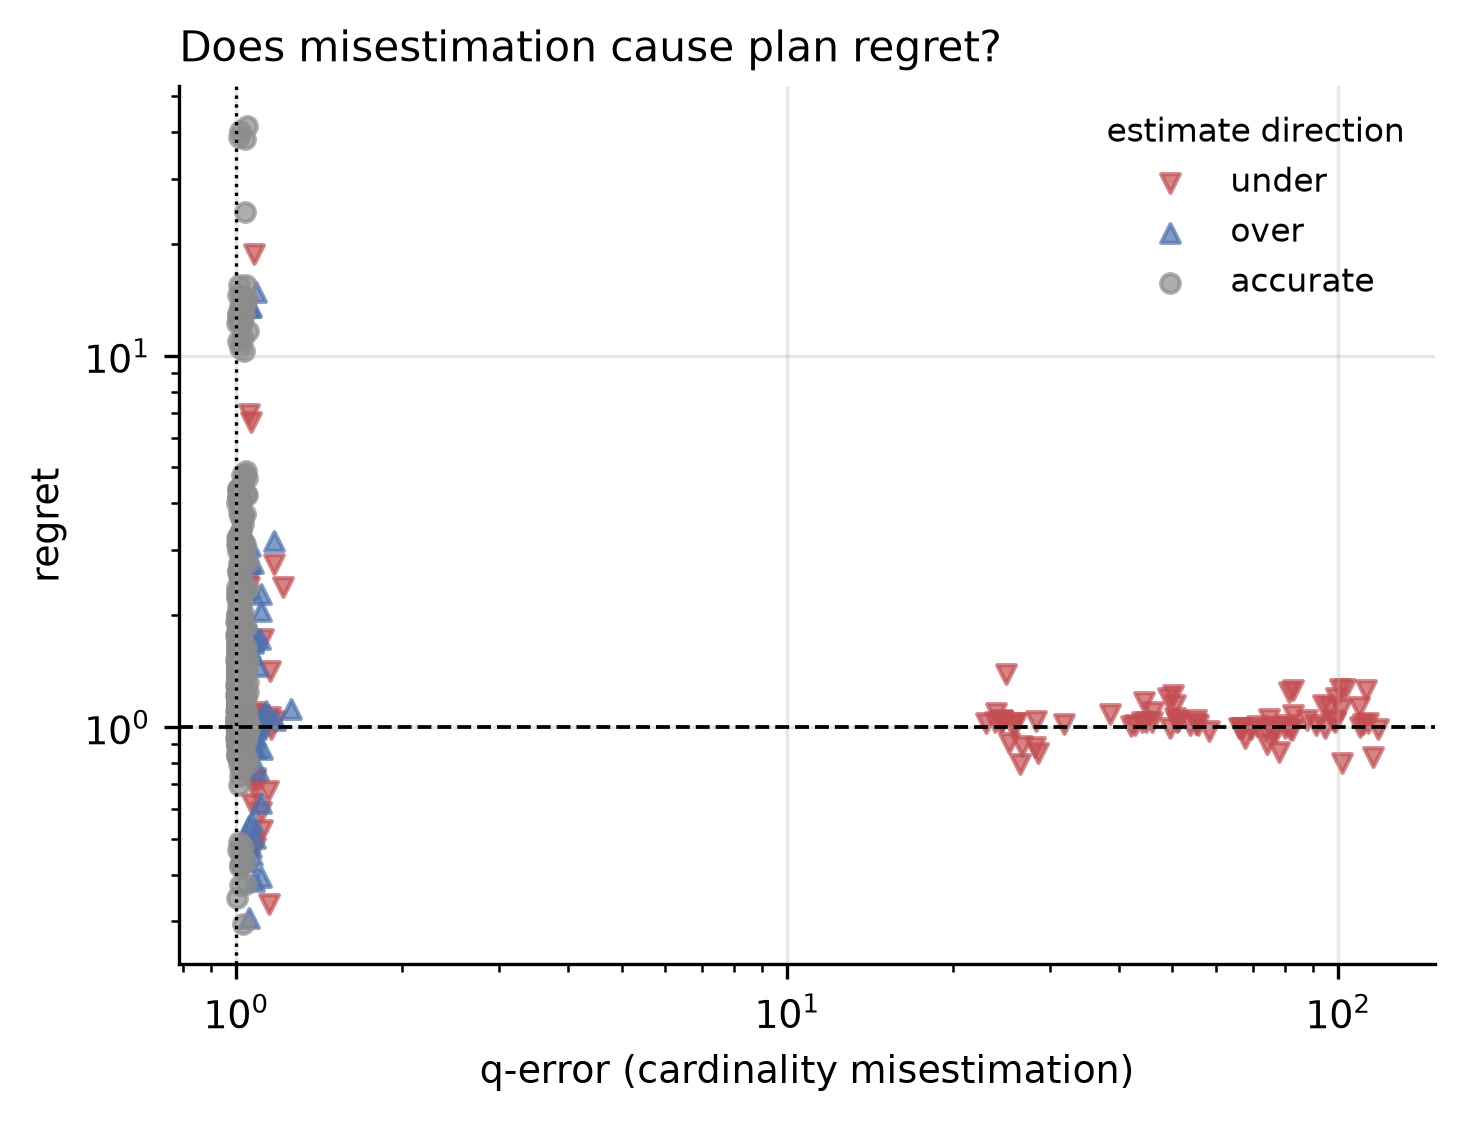
\includegraphics[width=0.62\linewidth]{figures/fig3_qerror_vs_regret.png}
\caption{Access-path regret against cardinality estimation error, by
direction of the error. High-regret queries cluster at $q$-error near
one, so misestimation does not account for them.}
\label{fig:qerror}
\end{figure}

We regard this as the paper's most important negative result. It
excludes the explanation that \citet{leis2015good} would suggest and
directs attention to the cost model and to path generation. The
divergence from their finding is explicable: join ordering has a
combinatorially large plan space in which small estimation errors
compound, whereas access-path selection has three or four candidates
and no compounding, so cost-model calibration and path enumeration
dominate instead.

\subsection{RQ4a: extended statistics}
\label{sec:extstats}

\texttt{CREATE STATISTICS} is the documented remedy for correlated
predicates \citep{pgdocs17createstats}. It succeeds at its stated
objective and degrades the outcome (Table~\ref{tab:extstats},
Figure~\ref{fig:extstats}).

\begin{table}[htbp]
\centering
\caption{Effect of extended statistics on dependent conjunctive
predicates at $10^6$ rows. Estimates become nearly exact; every
affected query becomes slower.}
\label{tab:extstats}
\small
\begin{tabular}{@{}lrrrrrrr@{}}
\toprule
Dependency & \multicolumn{2}{c}{$q$-error} & Est.\ rows & True & \multicolumn{2}{c}{Median ms} & Slow- \\
\cmidrule(lr){2-3}\cmidrule(lr){6-7}
strength & without & with & with & rows & without & with & down \\
\midrule
0.25 & 25.23 & 1.11 & 2{,}767 & 2{,}556 & 0.93 & 2.54 & 2.73$\times$ \\
0.50 & 49.52 & 1.04 & 5{,}200 & 5{,}053 & 2.12 & 3.53 & 1.66$\times$ \\
0.75 & 75.89 & 1.02 & 7{,}633 & 7{,}513 & 2.80 & 4.34 & 1.55$\times$ \\
1.00 & 113.19 & 1.05 & 9{,}700 & 9{,}995 & 3.95 & 5.06 & 1.28$\times$ \\
\bottomrule
\end{tabular}
\end{table}

\begin{figure}[htbp]
\centering
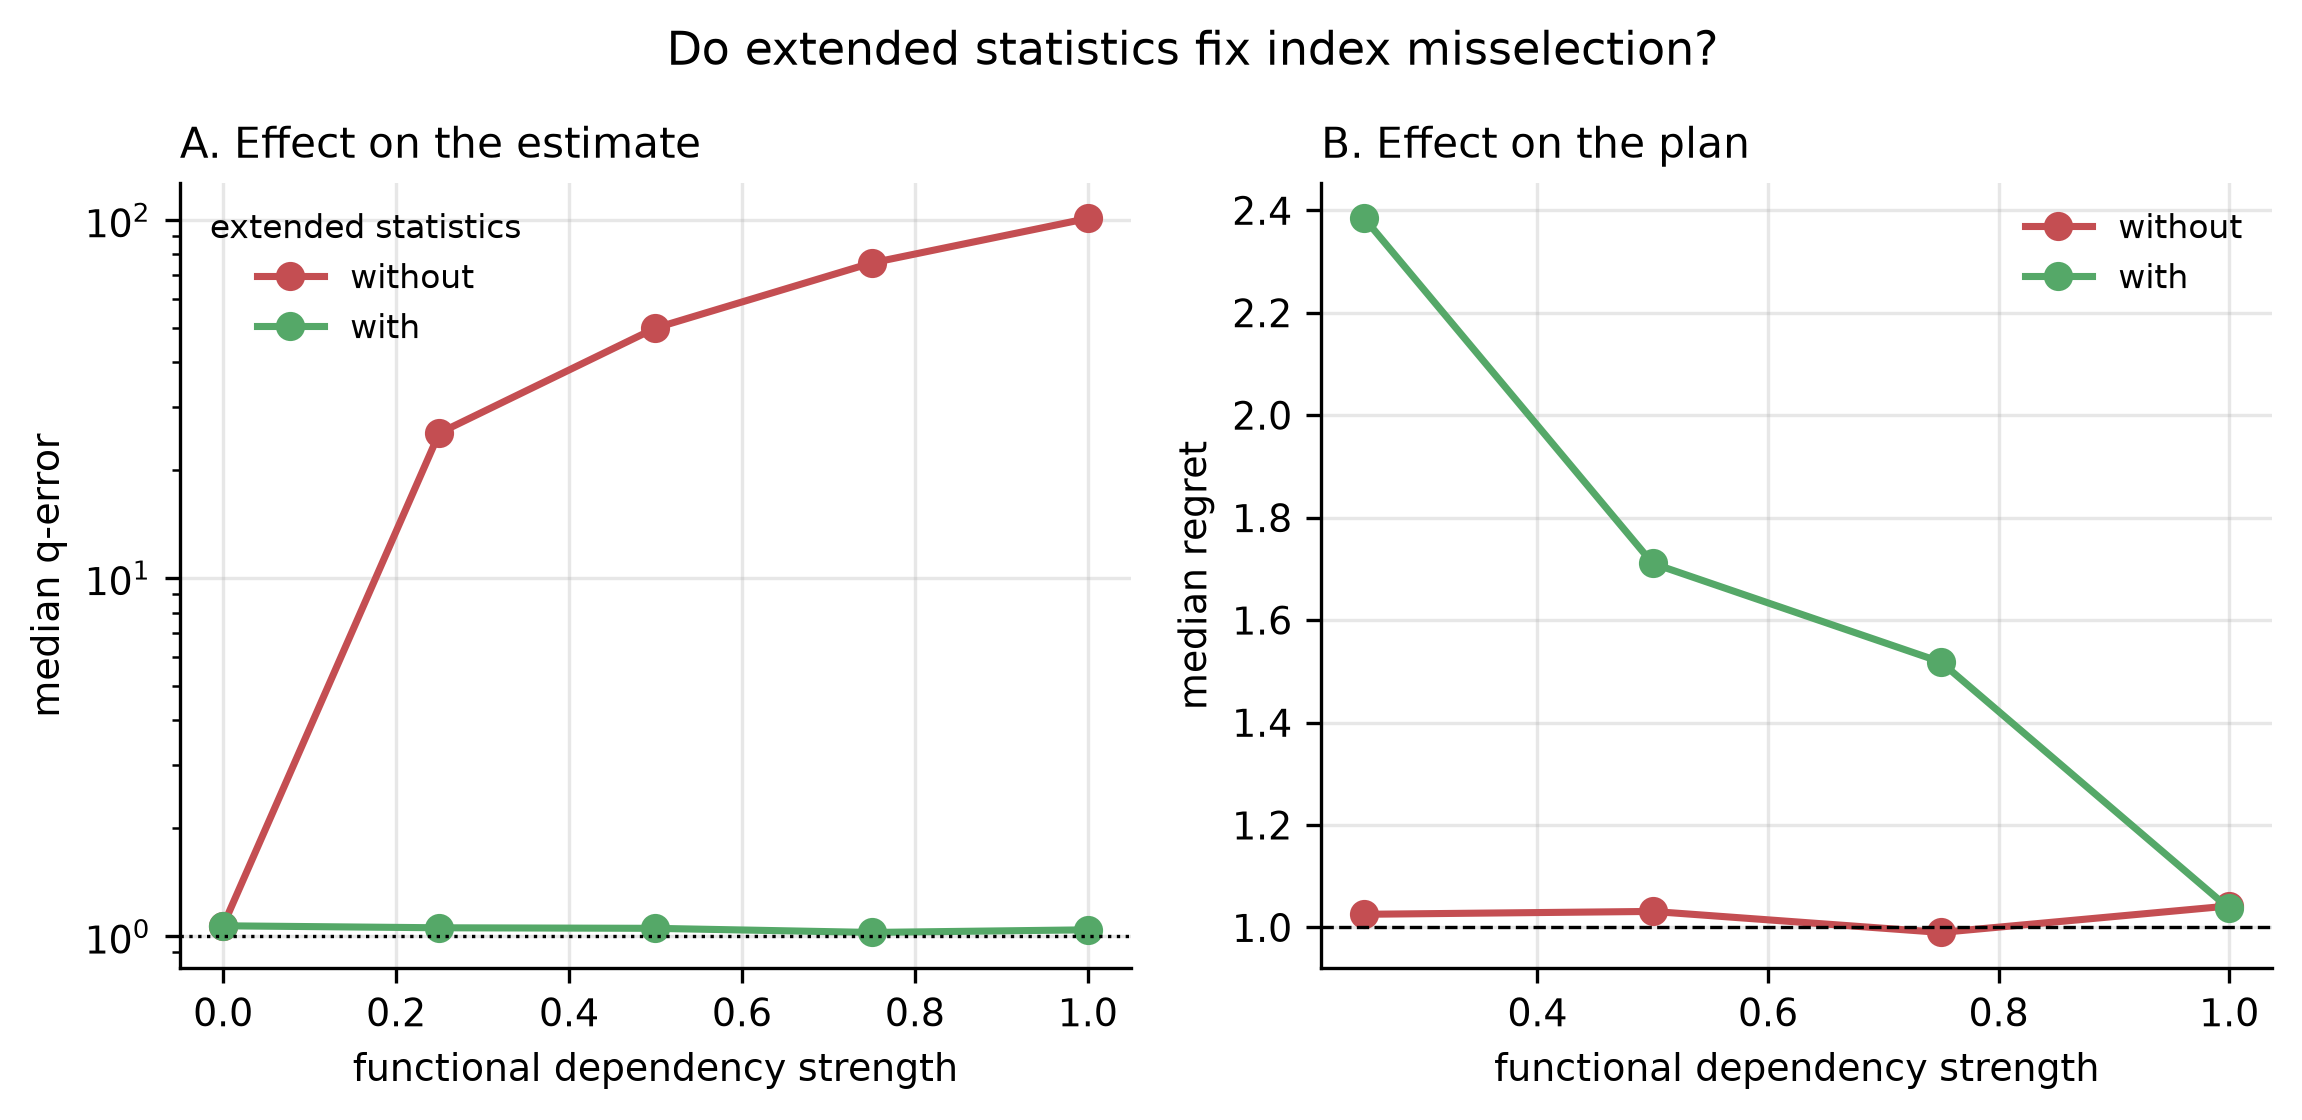
\includegraphics[width=0.95\linewidth]{figures/fig4_extended_statistics.png}
\caption{Extended statistics against dependency strength. Panel A: the
estimate improves by up to two orders of magnitude. Panel B: the
resulting plan degrades. Improving the estimate and improving the plan
are separable outcomes.}
\label{fig:extstats}
\end{figure}

\paragraph{Mechanism}
Without extended statistics the optimiser uses the composite index on
$(a, b)$ in a single index scan. With them it switches to a
\texttt{BitmapAnd} over two single-column indexes. Both plans fetch the
identical 7{,}317 heap blocks, but the second performs two index scans
plus a bitmap intersection in place of one scan. The reason for the
switch is visible in the node-level estimates:

\begin{lstlisting}[caption={Node row estimates with extended statistics present.}]
Bitmap Heap Scan  ... rows=10367     <- extended statistics applied
  -> BitmapAnd    ... rows=107       <- independence assumption, not corrected
\end{lstlisting}

Since $10367^2 / 10^6 \approx 107$, the \texttt{BitmapAnd} node is
still multiplying per-column selectivities under exactly the
independence assumption that extended statistics exist to replace. The
optimiser consequently prices the \texttt{BitmapAnd} at 635 using the
uncorrected figure and the composite path at 13{,}558 using the
corrected one, a 21-fold discrepancy, and selects the plan that is in
fact slower.

We verified that the optimiser is behaving rationally given its own
model by restricting the available indexes. With only the composite
index present and extended statistics active, that path is priced at
13{,}558 yet executes in 4.030\,ms, faster than the
\texttt{BitmapAnd} at 4.794\,ms. Without extended statistics the same
composite path is priced at 392.80 and executes in 4.155\,ms. The
corrected estimate therefore makes an equally fast plan appear
34$\times$ more expensive. The defect is not the optimiser's choice
procedure but the inconsistent propagation of the correction across
path types.

\subsection{RQ4b: reducing \rpc{}}
\label{sec:rpc}

The default \rpc{} of 4.0 encodes a magnetic-disk assumption, and
guidance widely recommends reducing it on flash storage. Measured
across the full query set, the recommendation is counterproductive in
our environment (Table~\ref{tab:rpc}, Figure~\ref{fig:rpc}).

\begin{table}[htbp]
\centering
\caption{Total execution time over the full query set at each \rpc{},
conventional index set.}
\label{tab:rpc}
\small
\begin{tabular}{@{}lrr@{}}
\toprule
\rpc{} & Total time (ms) & Versus best \\
\midrule
1.0 & 2{,}306 & 2.3$\times$ worse \\
1.1 & 1{,}954 & 1.9$\times$ worse \\
1.2 & 1{,}942 & 1.9$\times$ worse \\
1.5 & 1{,}006 & best \\
2.0 & 1{,}053 & 1.0$\times$ \\
3.0 & 1{,}053 & 1.0$\times$ \\
4.0 (default) & 1{,}068 & 1.06$\times$ \\
\bottomrule
\end{tabular}
\end{table}

\begin{figure}[htbp]
\centering
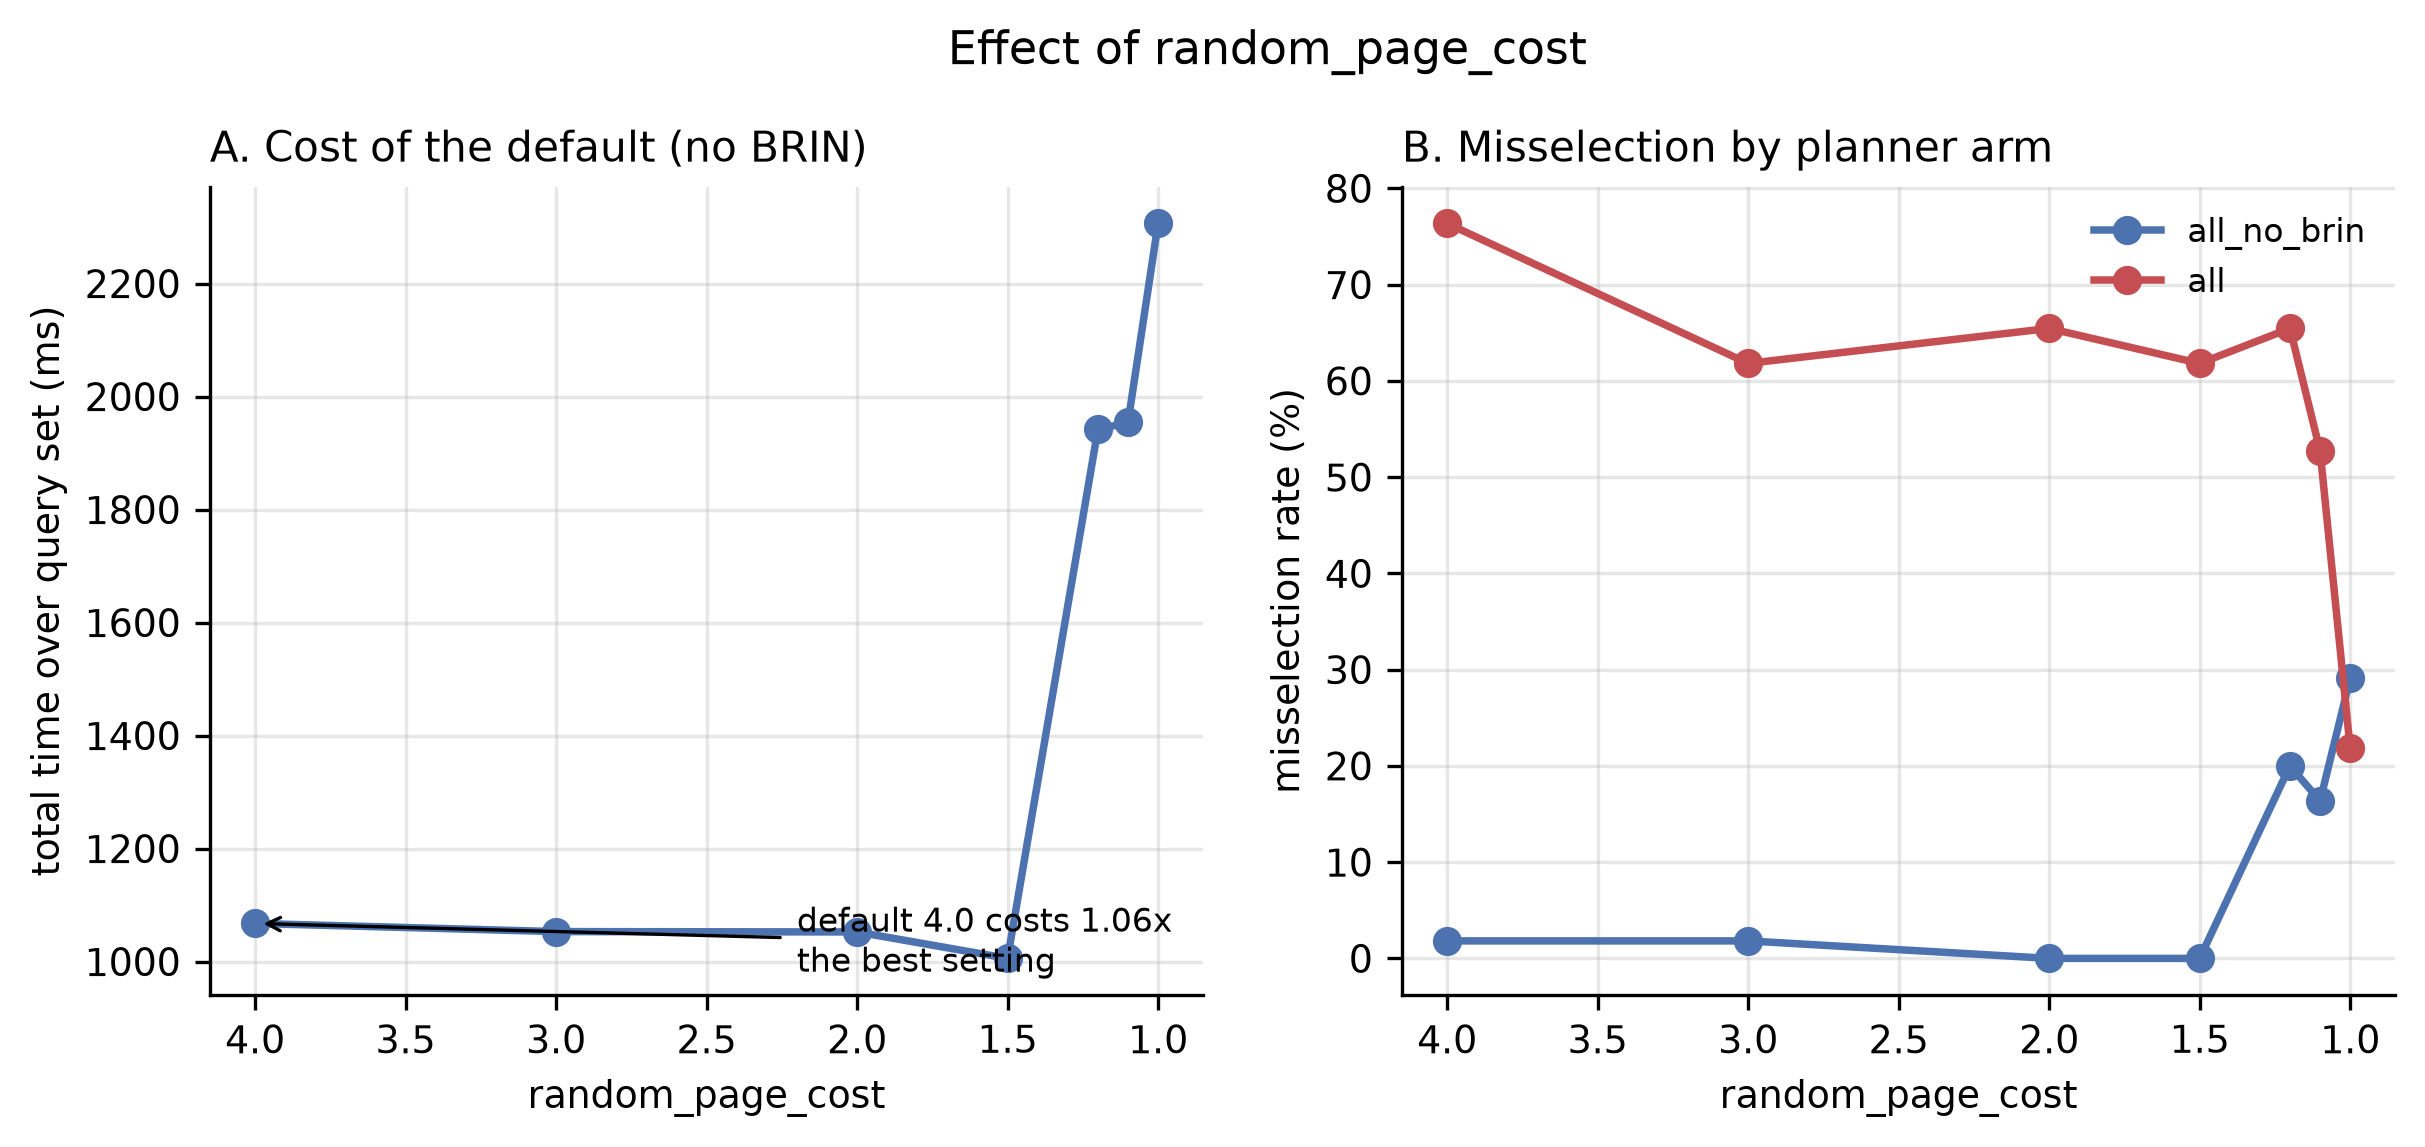
\includegraphics[width=0.95\linewidth]{figures/fig6_random_page_cost.png}
\caption{Effect of \rpc{}. Panel A: total query-set time; reducing the
setting below 1.5 degrades the workload. Panel B: misselection rate by
index configuration.}
\label{fig:rpc}
\end{figure}

The default lies within 6\% of optimal. Reducing it to 1.0 costs a
factor of 2.3. Access-path counts explain the mechanism: at
$\rpc = 1.0$ the optimiser abandons bitmap scans entirely in favour of
plain index scans, 136 index scans against zero bitmap scans, which is
the wrong choice for higher-selectivity predicates because it forfeits
the physical-order sorting that makes bitmap heap access efficient.

A single-query measurement early in this study indicated the default
cost 24$\times$ (Table~\ref{tab:rpcsingle}). That observation was
accurate but unrepresentative. We retain it as a documented instance of
how anecdotal tuning evidence misleads, a pattern
\citet{raasveldt2018fair} identify as endemic.

\begin{table}[htbp]
\centering
\caption{Single-query sensitivity to \rpc{}, identical row estimate
(10{,}662) throughout. Compare with Table~\ref{tab:rpc}.}
\label{tab:rpcsingle}
\small
\begin{tabular}{@{}lrr@{}}
\toprule
\rpc{} & Plan chosen & Median ms \\
\midrule
4.0 (default) & sequential scan & 49.14 \\
2.0 & B-tree index scan & 2.08 \\
1.5 & B-tree index scan & 2.33 \\
1.1 & B-tree index scan & 2.49 \\
1.0 & B-tree index scan & 2.25 \\
\bottomrule
\end{tabular}
\end{table}

\subsection{RQ2 and RQ4c: a co-located BRIN index}
\label{sec:brin}

BRIN indexes are small and cheap to build, so adding one is commonly
regarded as harmless. It is not, while the table is buffer-pool
resident (Table~\ref{tab:brin}, Figure~\ref{fig:brinfig}).

\begin{table}[htbp]
\centering
\caption{Effect of adding a BRIN index alongside an existing B-tree on
the same column.}
\label{tab:brin}
\small
\begin{tabular}{@{}lrrrr@{}}
\toprule
Scale & With BRIN & Without BRIN & Median $R$ & Max $R$ \\
\midrule
$10^6$ & 73.3\% & 2.3\% & 2.06 vs 1.01 & 18.78 \\
$10^7$ & 30.1\% & 32.3\% & 1.04 vs 1.04 & 2.63 \\
\bottomrule
\end{tabular}
\end{table}

\begin{figure}[htbp]
\centering
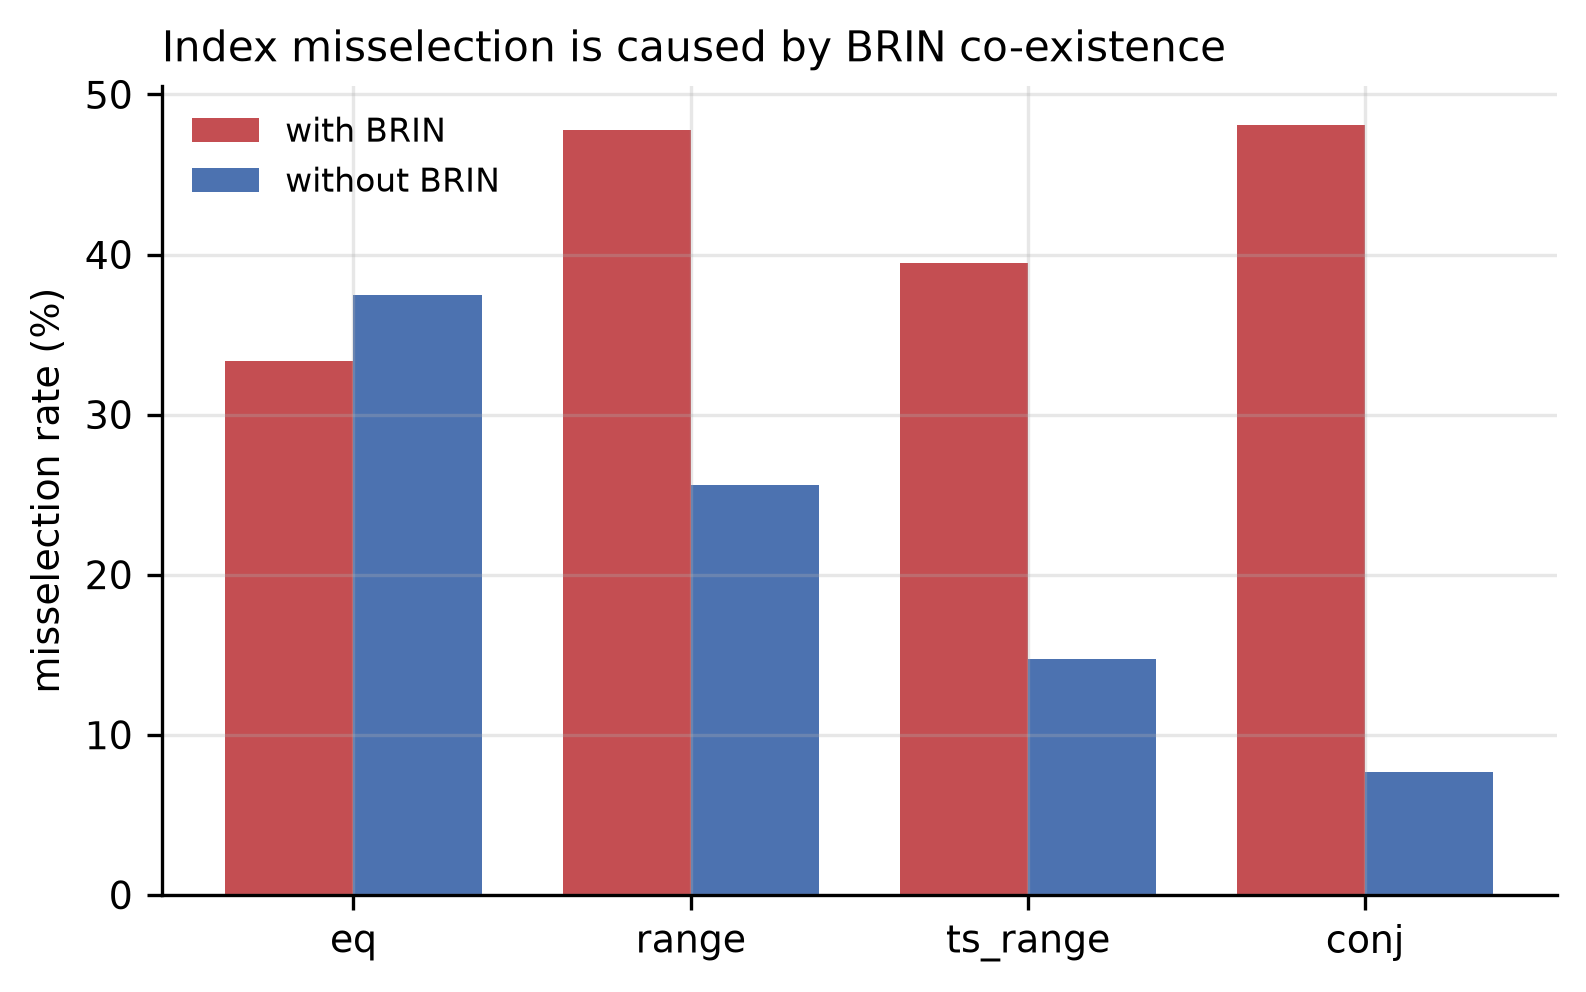
\includegraphics[width=0.66\linewidth]{figures/fig0_brin_effect.png}
\caption{Misselection rate by query family with and without BRIN in the
index set at $10^6$ rows. The conjunctive family is the control: no
BRIN index covers those columns and correspondingly no effect appears.}
\label{fig:brinfig}
\end{figure}

The conjunctive family serves as an internal control. No BRIN index
covers columns $a$ or $b$, and correspondingly the matched comparison
shows a median speedup of $0.90\times$ from removing BRIN for that
family, against $2.83\times$ and $2.78\times$ for the range families.
The effect appears exactly where the mechanism predicts it should.

\paragraph{Mechanism}
With both indexes present and a bitmap plan forced by disabling other
access methods, the optimiser selected BRIN in 16 of 16 cases, and in
ten of those the B-tree bitmap path was cheaper \emph{by the
optimiser's own cost model}, in one case by a factor of nine
(Table~\ref{tab:suppression}). A cost-based optimiser does not
knowingly select a path it prices as nine times more expensive, so the
B-tree bitmap path cannot be reaching the final comparison at all.

Inspection of the PostgreSQL~17 source confirms this and identifies the
responsible line. Bitmap path selection is performed by
\texttt{choose\_bitmap\_and()} in
\texttt{src/backend/optimizer/path/indxpath.c}. Before that function
performs its greedy cost comparison, it deduplicates candidates,
described in the source comment as detecting ``any paths that use
exactly the same set of clauses'' and keeping ``only the
cheapest-to-scan of any such groups''. A BRIN index and a B-tree index
on the same column serving the same predicate use precisely the same
clause set, so they are classified as duplicates and only one survives.

The tiebreak is the critical detail. The surviving path is chosen by
\texttt{cost\_bitmap\_tree\_node()}, which returns the index path's
\texttt{indextotalcost}, that is the cost of the \emph{index-side} scan
alone. It does not consider the bitmap heap scan that consumes the
resulting bitmap. Only after deduplication does the function evaluate
full scan cost, via \texttt{bitmap\_scan\_cost\_est()}, and by then the
discarded path is gone.

This makes the failure systematic rather than incidental. BRIN's entire
design goal is a very small index, so its index-side cost is
necessarily far below a B-tree's; in our measurements 12.13 against
213.35 for the same predicate. BRIN therefore wins the tiebreak
essentially by construction. Yet the whole cost difference between the
two plans lies on the heap side, which the tiebreak does not examine:
the B-tree bitmap is exact while the BRIN bitmap is lossy at block
granularity, forcing the recheck of 990{,}000 rows documented below.
The deduplication selects on the one metric on which BRIN always wins,
and ignores the metric on which it can lose by two orders of magnitude.

We emphasise that this is a cost-model layering issue rather than a
coding error. Deduplicating equivalent paths is sound, and using a
cheap proxy to break ties is reasonable when candidate paths have
comparable heap behaviour, as two B-trees would. It ceases to be
reasonable when index structures differ in bitmap precision, which is
exactly what BRIN introduced.

\begin{table}[htbp]
\centering
\caption{Forced bitmap plans with both indexes present, statistics held
byte-identical within each row. BRIN is selected in every case.}
\label{tab:suppression}
\small
\begin{tabular}{@{}llrrrr@{}}
\toprule
Corr. & Query & BRIN cost & BRIN ms & B-tree cost & B-tree ms \\
\midrule
0.0 & 0.1\% range & 29{,}320 & 65.95 & 3{,}166 & 0.34 \\
0.0 & 1\% range & 29{,}322 & 66.73 & 13{,}857 & 5.14 \\
0.5 & 0.1\% range & 15{,}338 & 66.33 & 3{,}174 & 0.21 \\
0.5 & 1\% range & 14{,}852 & 63.90 & 13{,}848 & 2.76 \\
0.95 & 0.1\% range & 13{,}511 & 62.07 & 3{,}294 & 0.09 \\
0.95 & 1\% range & 15{,}365 & 66.45 & 14{,}201 & 0.76 \\
\bottomrule
\end{tabular}
\end{table}

The execution cost of the selected plan is visible in its profile:
\texttt{Heap Blocks: lossy=14304} with
\texttt{Rows Removed by Index Recheck: 990000}. The BRIN path reads
essentially the entire table and discards 99\% of what it reads. The
largest penalty observed is the 0.95-correlation, 0.1\% selectivity
case: 62.07\,ms against 0.09\,ms, a factor of 690.

\subsection{RQ5: locating the boundaries}
\label{sec:boundary}

Comparing $10^6$ against $10^7$ rows shows the penalty present at the
smaller scale and absent at the larger. Two points, however, cannot
distinguish gradual decay from a sharp transition, nor reveal
non-monotonic behaviour between them. We therefore measured five
intermediate scales (Table~\ref{tab:transition},
Figure~\ref{fig:transition}).

\begin{table}[htbp]
\centering
\caption{The BRIN penalty across table size. Frequency and severity
collapse at different scales.}
\label{tab:transition}
\small
\begin{tabular}{@{}rrrrrrr@{}}
\toprule
Million & Heap & Blocks read & \multicolumn{2}{c}{Misselection \%} & \multicolumn{2}{c}{Max regret} \\
\cmidrule(lr){4-5}\cmidrule(lr){6-7}
rows & (MB) & outside pool & with BRIN & without & with BRIN & without \\
\midrule
1.00 & 111.8 & 0 & 71.4 & 0.0 & 18.78 & 1.06 \\
1.25 & 139.8 & 0 & 37.9 & 34.5 & 38.81 & 1.67 \\
1.50 & 167.8 & 0 & 31.0 & 17.2 & 40.32 & 1.76 \\
2.00 & 223.2 & 0 & 25.8 & 12.9 & 38.34 & 1.77 \\
3.00 & 335.2 & 0 & 30.3 & 12.1 & 41.51 & 1.67 \\
5.00 & 558.2 & 1{,}902 & 36.4 & 30.3 & 6.98 & 1.81 \\
10.00 & 1{,}116.2 & 89{,}081 & 38.2 & 44.4 & 1.92 & 3.70 \\
\bottomrule
\end{tabular}
\end{table}

\begin{figure}[htbp]
\centering
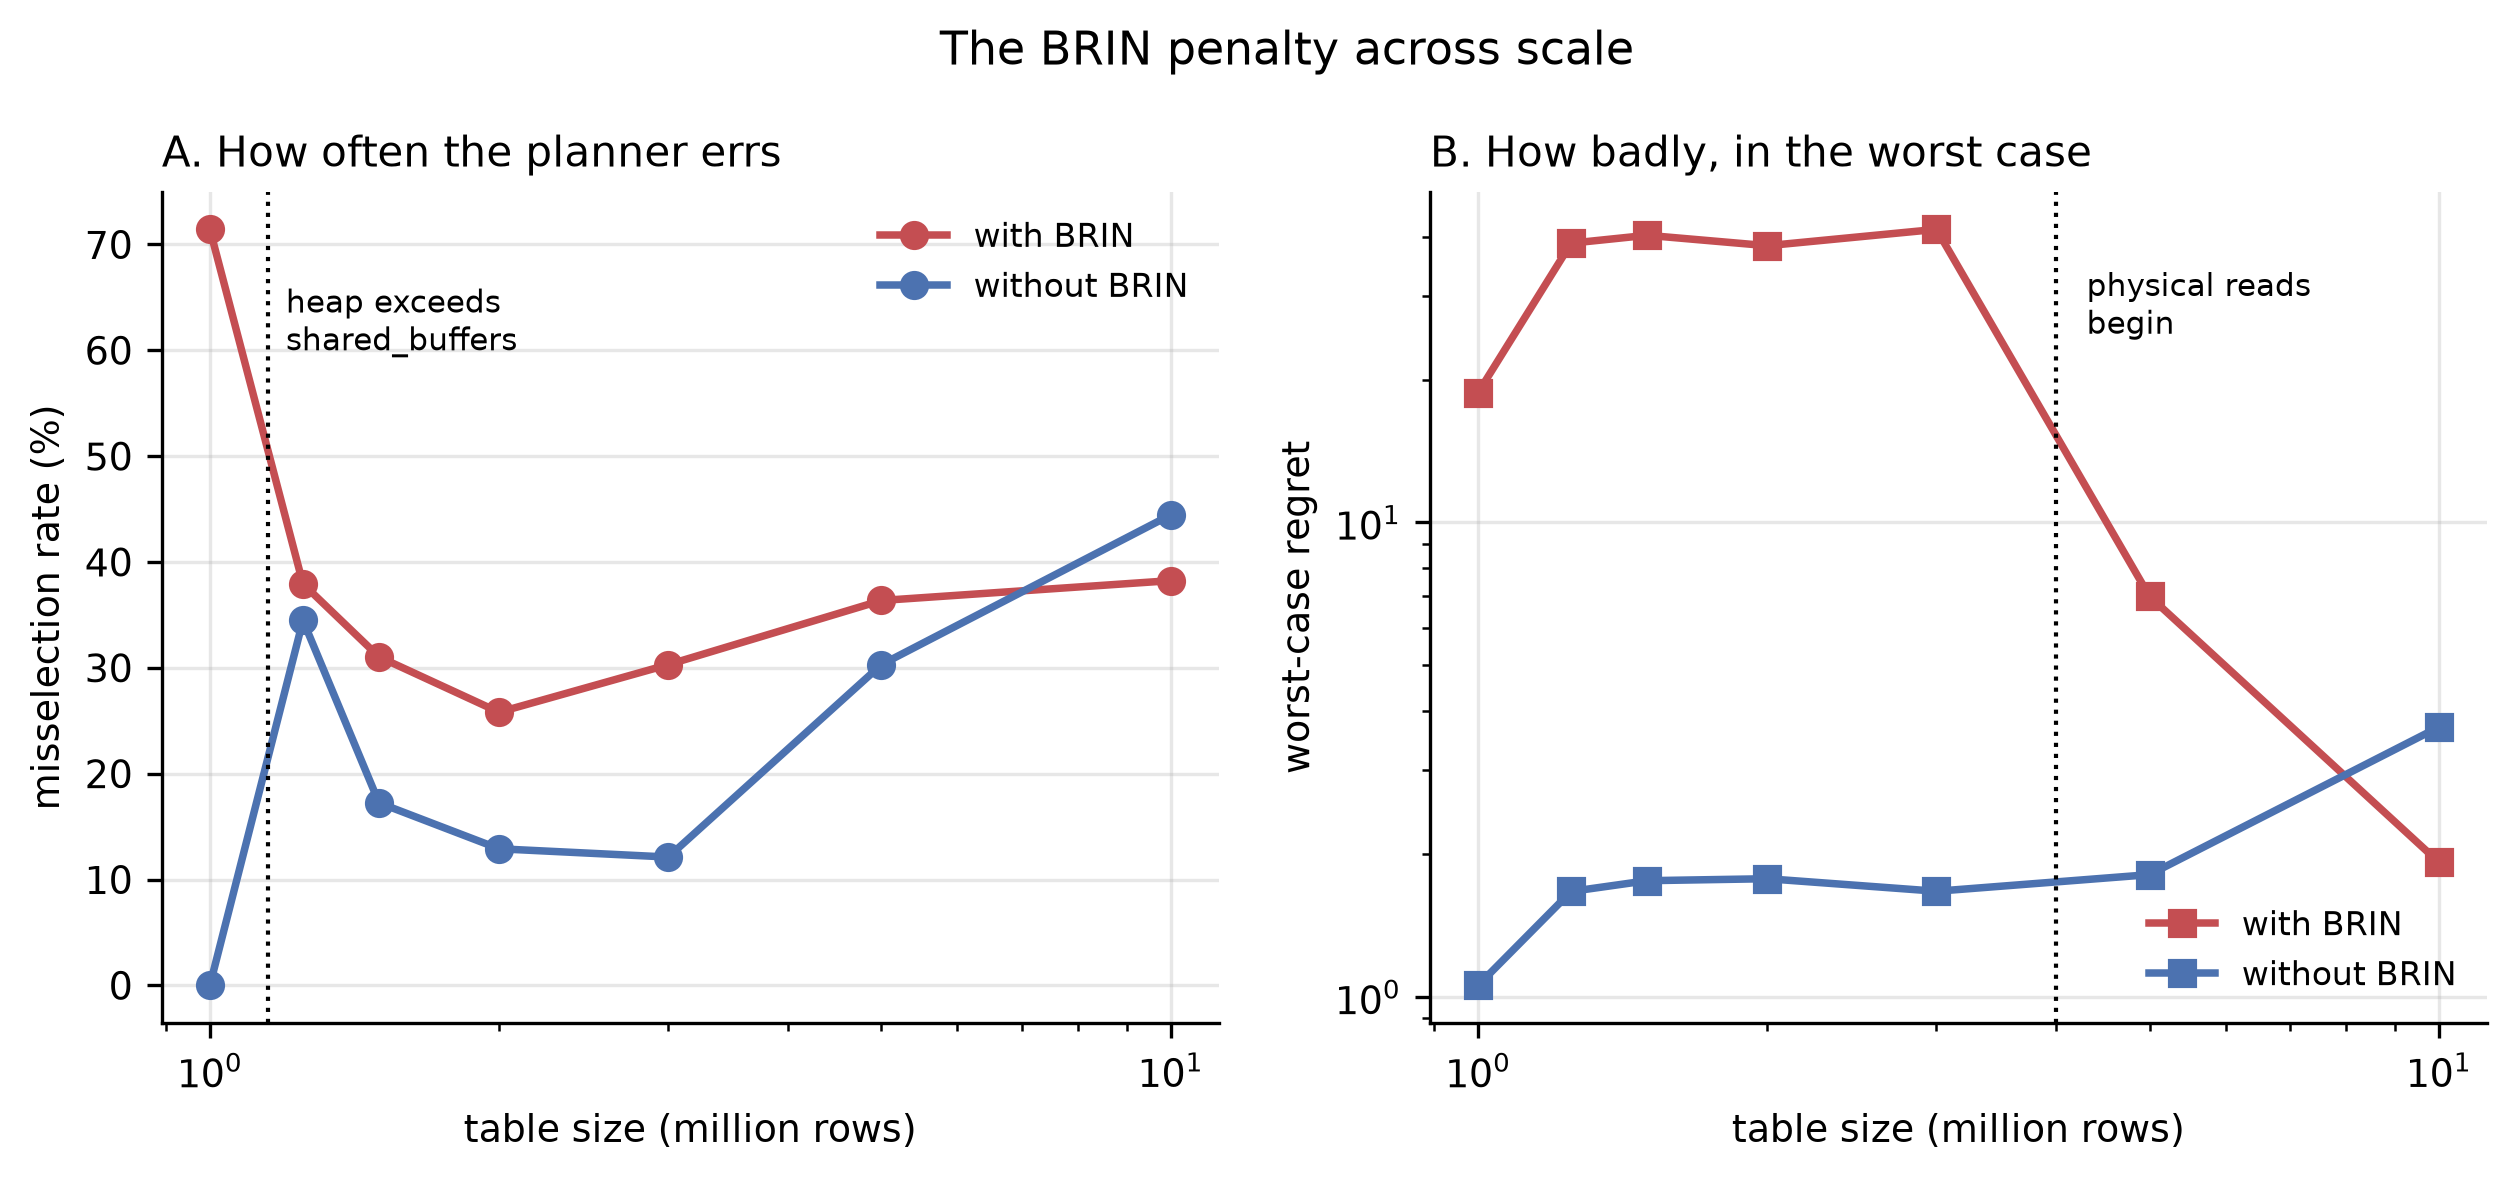
\includegraphics[width=0.95\linewidth]{figures/fig7_scale_transition.png}
\caption{The BRIN penalty across scale. Panel A: how often the
optimiser errs. Panel B: worst-case regret. The two collapse at
different table sizes, near different system boundaries.}
\label{fig:transition}
\end{figure}

There are two transitions, not one.

\paragraph{Frequency collapses at the buffer pool boundary}
The gap in misselection rate falls from 71.4 percentage points at
$10^6$ rows to 3.4 at $1.25 \times 10^6$. That is precisely where the
heap crosses \sbuf{}: 111.8\,MB against a 128\,MB pool becomes
139.8\,MB. The composition of the collapse is instructive. The
BRIN-inclusive configuration improves from 71.4\% to 37.9\%, but the
conventional configuration \emph{degrades} from 0.0\% to 34.5\%. The
gap closes principally because the baseline deteriorates once the
working set no longer fits, not because BRIN improves.

\paragraph{Severity collapses later, after first intensifying}
Worst-case regret with BRIN does not decline past the buffer pool
boundary. It approximately doubles, from 18.78 at $10^6$ rows to 38.81
at $1.25 \times 10^6$, and remains near 40 through $3 \times 10^6$. It
falls only at $5 \times 10^6$ (6.98) and $10^7$ (1.92). That later
collapse coincides with the onset of physical reads: blocks fetched
from outside the buffer pool are zero up to $3 \times 10^6$ rows,
1{,}902 at $5 \times 10^6$ and 89{,}081 at $10^7$.

The practical implication inverts the naive reading. A deployment whose
table is two to three times \sbuf{} experiences the most severe
individual regressions measured anywhere in this study, worse than at
the scale where the effect was first identified. Had we reported only
the two-point comparison, we would have concluded that the penalty
diminishes with scale and implicitly reassured exactly the
practitioners most at risk.

We do not claim a verified causal mechanism for either transition. What
is established is that each coincides with a specific, independently
measurable system boundary, and that the two boundaries are distinct.

\subsection{RQ6: which findings generalise?}
\label{sec:crossdbms}

A single-system study cannot separate properties of cost-based
access-path selection from artefacts of one implementation. We
therefore repeated the $10^6$-row sweep on MariaDB~10.4.28 using the
same generated data, the same queries and the same regret metric,
with \texttt{innodb\_buffer\_pool\_size} set to 128\,MB to match
PostgreSQL's \sbuf{}. The comparison is restricted to the six index
configurations both systems support; InnoDB offers neither BRIN nor
hash indexes, so those PostgreSQL arms have no counterpart and the
BRIN result of Section~\ref{sec:brin} cannot be replicated at all.
Measurement used \texttt{ANALYZE FORMAT=JSON}, MariaDB's equivalent of
\texttt{EXPLAIN ANALYZE}.

\paragraph{Selection quality does not generalise}
On identical data and queries the two optimisers differ sharply
(Table~\ref{tab:crossdbms}). PostgreSQL misselects for 2.3\% of
queries, MariaDB for 66.0\%. MariaDB errs far more often but far more
mildly: median regret 1.34 against 1.01, worst case 7.91 against 1.39.

\begin{table}[htbp]
\centering
\caption{Same data, same queries, same metric, $10^6$ rows, arms common
to both systems.}
\label{tab:crossdbms}
\small
\begin{tabular}{@{}lrrrrr@{}}
\toprule
System & Queries & Misselection & Median $R$ & p90 $R$ & Max $R$ \\
\midrule
PostgreSQL 17.1 & 130 & 2.3\% & 1.013 & 1.13 & 1.39 \\
MariaDB 10.4.28 & 153 & 66.0\% & 1.341 & 2.43 & 7.91 \\
\bottomrule
\end{tabular}
\end{table}

The chosen plans explain the difference. PostgreSQL selects bitmap
scans almost everywhere, which sort matching tuple identifiers into
physical order and thereby convert random heap access into something
closer to sequential access. MariaDB has no equivalent intermediate
strategy for a single-index predicate: it either performs a
\texttt{ref} lookup or scans the table. It fell back to a full scan for
33 of the range queries and 33 of the timestamp-range queries, where
PostgreSQL used none. The absence of the bitmap middle ground, rather
than worse decision-making per se, accounts for most of the gap.

\paragraph{The correlated-predicate failure does generalise}
The more consequential comparison concerns conjunctive predicates
(Table~\ref{tab:crossconj}). MariaDB estimates them \emph{exactly},
$q$-error $1.0$, at dependency strengths 0.25 through 0.75, precisely
where PostgreSQL is wrong by factors of 26 to 82.

\begin{table}[htbp]
\centering
\caption{Median $q$-error on dependent conjunctive predicates. MariaDB
is exact until it switches plan shape.}
\label{tab:crossconj}
\small
\begin{tabular}{@{}lrrl@{}}
\toprule
Dependency strength & PostgreSQL & MariaDB & MariaDB plan \\
\midrule
0.25 & 26.39 & \textbf{1.00} & \texttt{ref} on composite index \\
0.50 & 49.01 & \textbf{1.00} & \texttt{ref} on composite index \\
0.75 & 81.82 & \textbf{1.00} & \texttt{ref} on composite index \\
1.00 & 98.65 & \textbf{55.84} & \texttt{index\_merge} \\
\bottomrule
\end{tabular}
\end{table}

\begin{figure}[htbp]
\centering
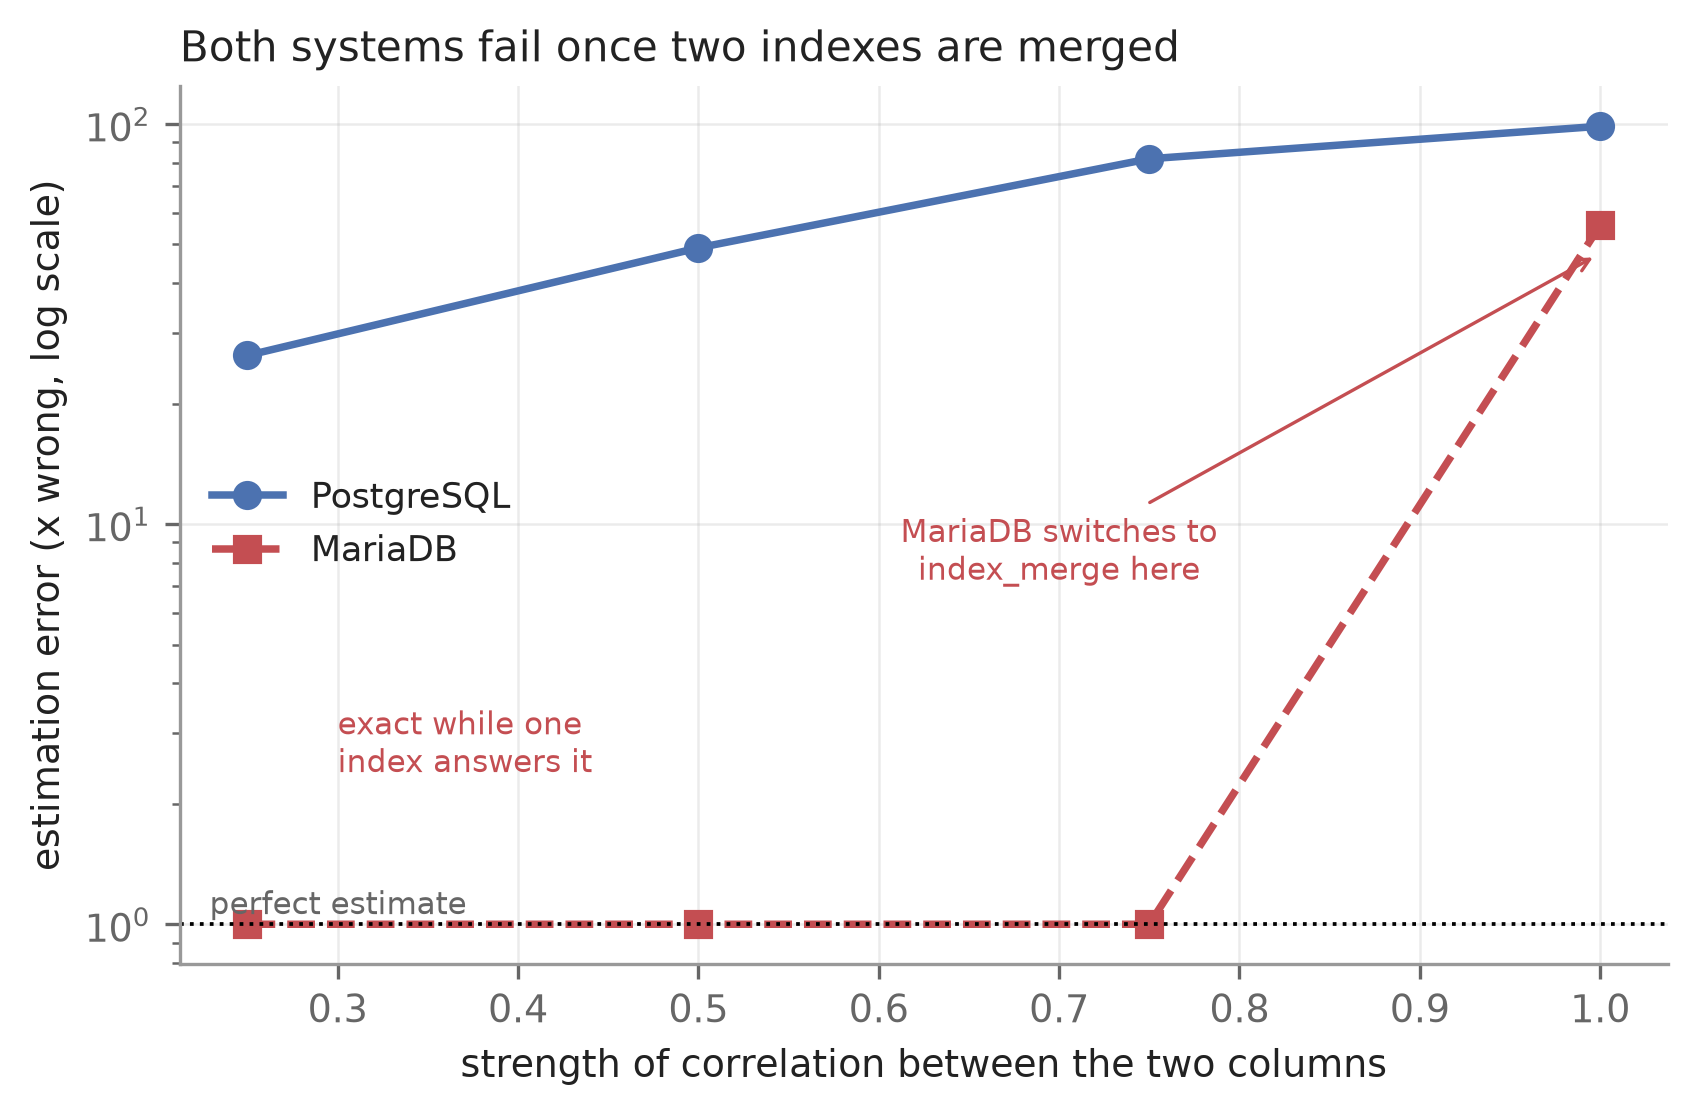
\includegraphics[width=0.70\linewidth]{figures/fig10_cross_conj.png}
\caption{Estimation error on dependent conjunctive predicates. MariaDB
is exact, and therefore flat on the dotted line, for as long as a single
composite index answers the predicate. Its error appears at the moment
it switches to \texttt{index\_merge}, reaching the same regime
PostgreSQL occupies throughout. Logarithmic vertical axis.}
\label{fig:crossconj}
\end{figure}

MariaDB achieves this through index dives. With both key parts of the
composite index bound it descends the B-tree and counts the qualifying
range rather than applying an independence assumption, so it measures
where PostgreSQL estimates. We confirmed the estimate is genuine and
not an artefact of the instrument by issuing \texttt{EXPLAIN
FORMAT=JSON}, which does not execute the query and nonetheless reports
the exact figure.

The decisive observation is what happens at full dependency. MariaDB
abandons the composite index for \texttt{index\_merge} over two
single-column indexes and its estimate immediately collapses, with
$q$-errors between 30 and 104 across the five queries.
\texttt{index\_merge} is the direct analogue of PostgreSQL's
\texttt{BitmapAnd}: both combine per-index bitmaps, and both derive the
combined cardinality by multiplying per-column selectivities under
independence.

Both systems are therefore accurate while a single index answers the
predicate, and both fail once a merge combines per-column estimates.
That the same failure appears in two independently developed optimisers,
one of which is otherwise more accurate on exactly these predicates,
indicates the defect belongs to the merge plan shape rather than to
either codebase. This substantially strengthens the extended-statistics
result of Section~\ref{sec:extstats}: the inconsistent propagation we
identified in PostgreSQL's \texttt{BitmapAnd} is one instance of a
general weakness in how merge-style plans estimate conjunctions.

\paragraph{Aggregate resource cost}
Regret measures whether an optimiser chose well among the options open to it.
It deliberately says nothing about what those options cost in absolute
terms, and the two questions can diverge: an optimiser that always picks
the best of a poor set of plans scores a regret near 1 while still being
slow. We therefore also report total execution time, which is the
quantity a practitioner actually pays.

Table~\ref{tab:resourcecost} compares the two systems over all eleven
datasets at $10^7$ rows, restricted to the index configurations common
to both. Every repetition of every query is included, so this is
measured work rather than wall clock, which would be contaminated by
interruptions and by differing maintenance costs.

\begin{table}[htbp]
\centering
\caption{Total measured work at $10^7$ rows over the four datasets and
six index configurations common to both systems. The two systems have
opposite cost profiles.}
\label{tab:resourcecost}
\small
\begin{tabular}{@{}lrrr@{}}
\toprule
System & Query execution & Index construction & Records \\
\midrule
PostgreSQL 17.1 & 50.8 min & 45.6 min & 1{,}232 \\
MariaDB 10.4.28 & 781.8 min & 19.3 min & 1{,}232 \\
\midrule
Ratio & \textbf{15.4$\times$ slower} & \textbf{2.4$\times$ faster} & \\
\bottomrule
\end{tabular}
\end{table}

Two observations follow.

First, the execution gap is an order of magnitude, far larger than the
regret figures alone suggest. Regret for MariaDB was 1.34 at the median,
implying mild inefficiency, yet its total execution cost is 15.4$\times$
PostgreSQL's on identical data. The reconciliation is that MariaDB
usually chooses close to the best plan \emph{available to it}, and the
plans available to it are worse. Regret measures decision quality;
Table~\ref{tab:resourcecost} measures the consequence of the plan
repertoire itself. Reporting only the former would understate the
difference by an order of magnitude.

Second, the profiles invert. PostgreSQL divides its time almost evenly
between building indexes (45.6 min) and executing queries (50.8 min),
whereas MariaDB builds in 19.3 min and then spends over thirteen hours
querying, a ratio above forty to one. Counting the BRIN and hash
configurations that MariaDB cannot provide, PostgreSQL's construction
cost rises to 128.8 min and exceeds its own query cost outright; we
exclude them from Table~\ref{tab:resourcecost} because including them on
one side only would not be a comparison. Either way the direction is the
same: a study measuring only build cost, or only query cost, would rank
these two systems in opposite orders. This is a caution for
index-selection work that models index benefit while treating
construction as negligible \citep{kossmann2020magic}: which cost
dominates is not a property of the workload but of the system executing
it.

\begin{figure}[htbp]
\centering
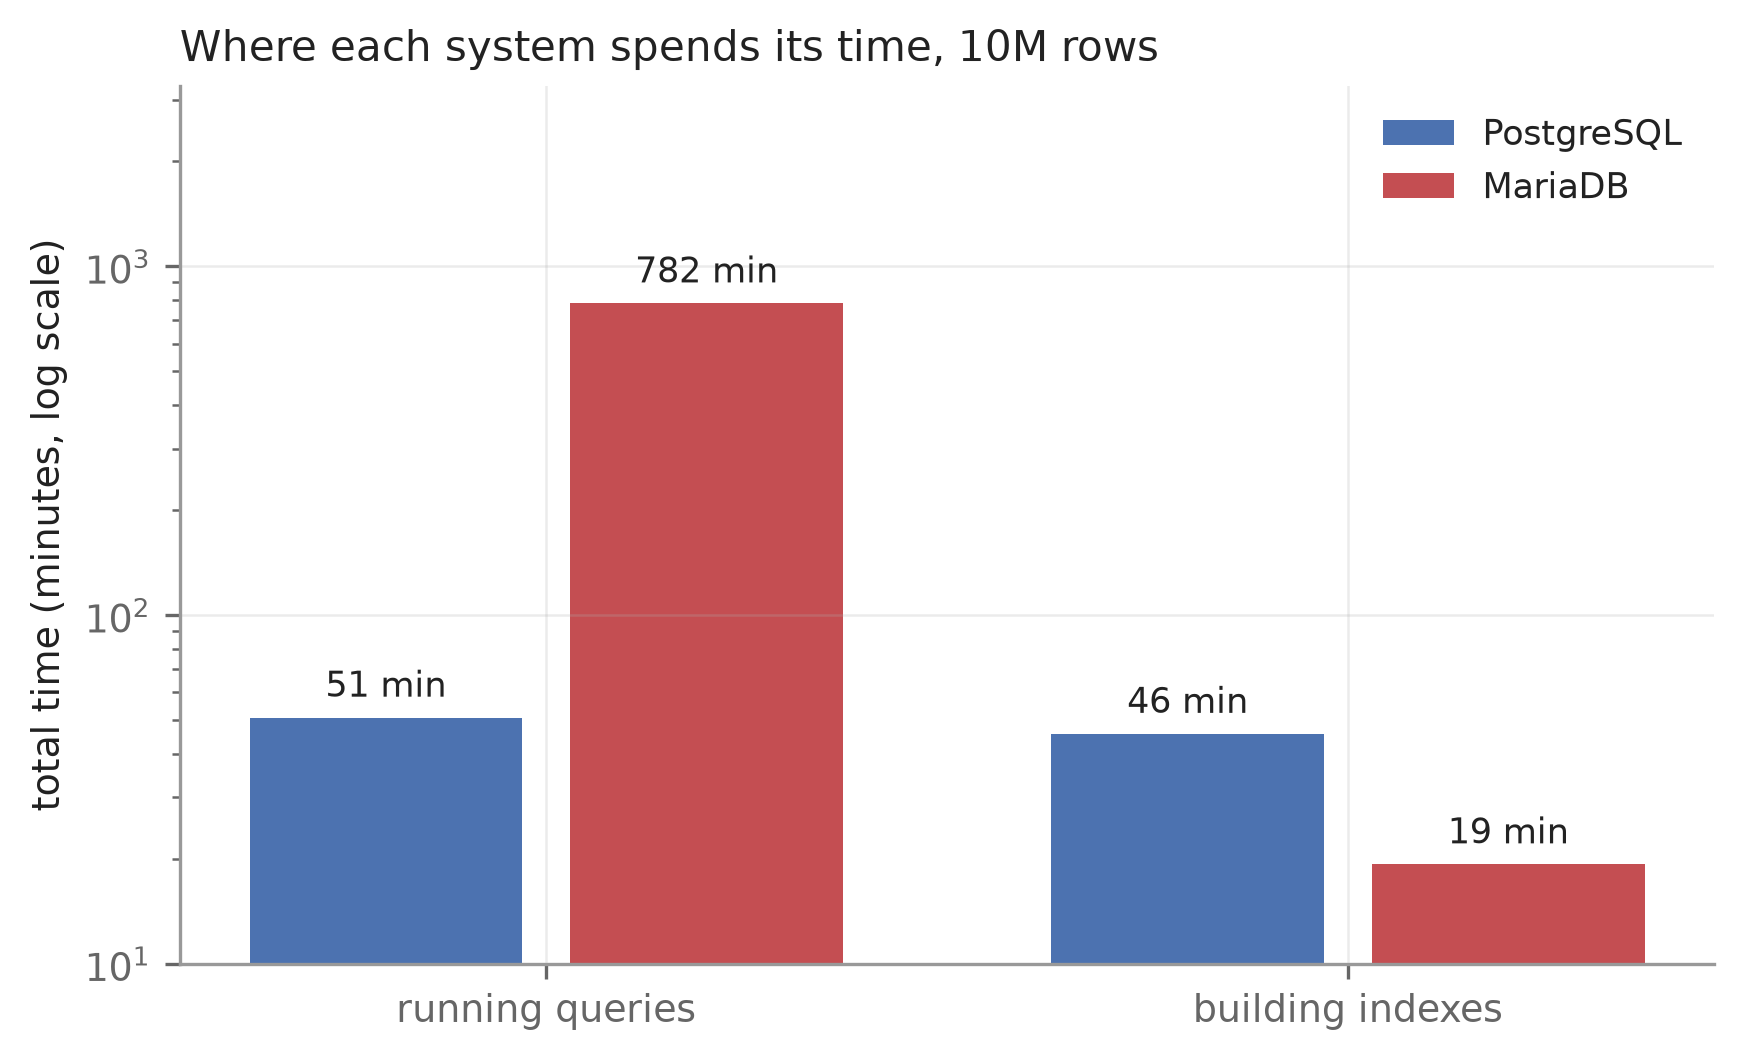
\includegraphics[width=0.72\linewidth]{figures/fig9_resource_cost.png}
\caption{Total measured work at $10^7$ rows, restricted to the index
configurations both systems provide. Note the logarithmic axis: the two
systems differ by more than an order of magnitude on query execution
while differing by rather less, in the opposite direction, on index
construction.}
\label{fig:resourcecost}
\end{figure}

\paragraph{Degradation has a different shape in each system}
Measuring both systems across the full scale range reveals that they do
not merely differ in degree, they degrade in opposite directions
(Table~\ref{tab:degradation}).

\begin{table}[htbp]
\centering
\caption{Both systems across scale, free-choice configuration,
\texttt{phys} datasets. The oracle for each system is restricted to the
index configurations both provide, so neither is credited with a plan
the other could not have formed. Misselection frequency and worst-case
severity move in opposite directions in the two systems.}
\label{tab:degradation}
\small
\begin{tabular}{@{}rrrrr@{}}
\toprule
Million & \multicolumn{2}{c}{PostgreSQL} & \multicolumn{2}{c}{MariaDB} \\
\cmidrule(lr){2-3}\cmidrule(lr){4-5}
rows & Misselection & Max $R$ & Misselection & Max $R$ \\
\midrule
1.00 & 0.0\% & 1.05 & 52.9\% & 3.33 \\
1.25 & 27.6\% & 1.67 & 74.3\% & 6.52 \\
1.50 & 6.9\% & 1.76 & 77.8\% & 10.85 \\
2.00 & 6.5\% & 1.36 & 75.7\% & 15.21 \\
3.00 & 6.1\% & 1.67 & 36.1\% & 18.77 \\
5.00 & 12.1\% & 1.80 & 37.9\% & 27.78 \\
10.00 & \textbf{36.1\%} & \textbf{3.70} & \textbf{12.4\%} & \textbf{30.85} \\
\bottomrule
\end{tabular}
\end{table}

\begin{figure}[htbp]
\centering
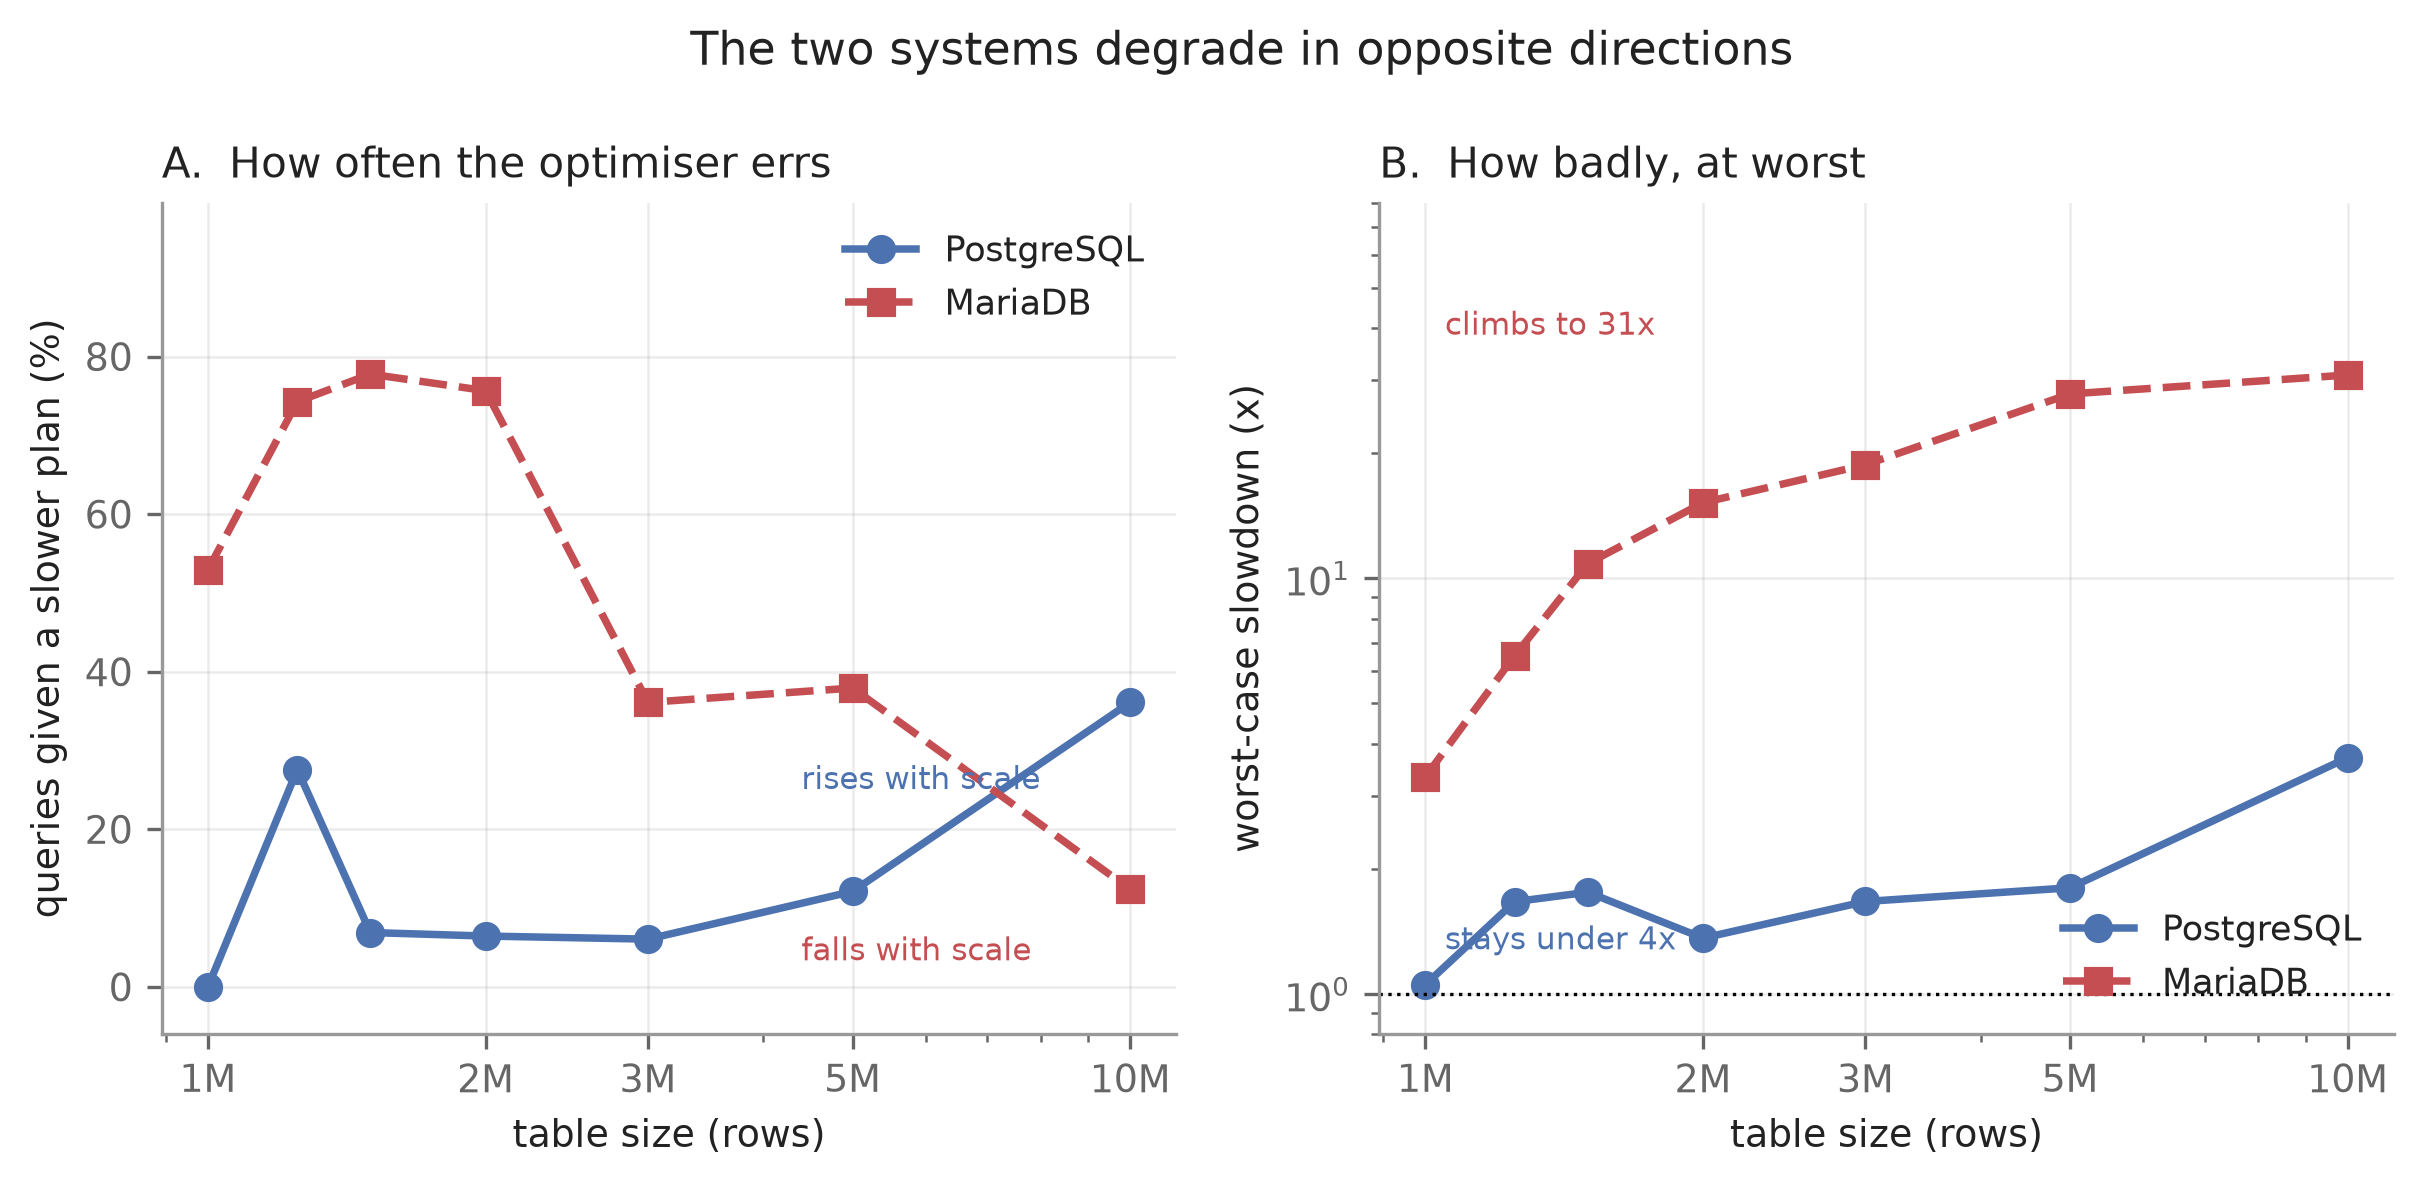
\includegraphics[width=0.98\linewidth]{figures/fig8_degradation_shape.png}
\caption{The same data as Table~\ref{tab:degradation}. Frequency and
severity are plotted on separate panels rather than a shared axis: they
carry different units, and placing them together would suggest a
relationship the data does not support. Panel B is logarithmic.}
\label{fig:degradation}
\end{figure}

PostgreSQL's misselection rate rises with scale, from 0\% to 36.1\%,
while its worst case stays bounded, never exceeding 3.7$\times$.
MariaDB's misselection rate falls with scale, from 52.9\% to 12.4\%,
while its worst case grows monotonically to 30.85$\times$. Each system
moves opposite to the other on both axes
(Figure~\ref{fig:degradation}).

A note on the oracle is warranted, because the comparison is sensitive
to it. Regret divides by the fastest configuration measured, so if
PostgreSQL's oracle included its BRIN configurations it would be judged
against plans MariaDB cannot form, and would appear worse than it is.
Restricting both oracles to the shared configurations changes
PostgreSQL's figures materially, at $1.5\times10^6$ rows from 17.2\% to
6.9\%, without altering the direction of either trend. We report the
restricted form throughout.

The interpretation follows from the plan repertoire. PostgreSQL errs
more often at scale but its bitmap intermediate bounds the cost of an
error: a wrong choice still reads the heap in physical order, so the
penalty is a constant factor rather than a collapse. MariaDB errs less
often at scale, because as the working set outgrows the buffer pool
fewer plans remain competitive and the choice becomes easier, but its
errors are unbounded, since a mistaken index scan degenerates into
random single-row fetches whose cost grows with the table.

This is a caution against summarising optimiser quality with a single
rate. An optimiser that is wrong 44\% of the time but never by more than
3.7$\times$ is preferable, for most workloads, to one that is wrong 12\%
of the time but occasionally by 31$\times$. Frequency and severity are
separate properties and, as these measurements show, they need not even
move in the same direction.

The mechanism is the one identified above. Lacking a bitmap intermediate,
MariaDB resolves an index match by fetching qualifying rows individually
in index order rather than in physical order. At $10^7$ rows the table and
its indexes total roughly 2\,GB against a 128\,MB buffer pool, so those
fetches miss the pool and become random device reads. Operating system
counters taken during the run confirm the interpretation: the MariaDB
process sat at 7.6\% CPU while sustaining 242\,MB/s of disk traffic with
the storage device at 71\% utilisation, that is, starved of I/O rather
than compute. Individual range queries that complete in milliseconds on
PostgreSQL reached 113 seconds.

\subsection{Incidental finding: hash index construction under skew}

Hash index build time proved acutely sensitive to value skew
(Table~\ref{tab:hashbuild}). Zipfian values collide into few hash
buckets, producing long overflow chains, and PostgreSQL does not
parallelise hash construction as it does B-tree construction. The
practical caution is that hash index creation cannot be assumed cheap
on skewed columns, a consideration absent from index-selection
tooling that models index benefit but not construction cost under
skew \citep{kossmann2020magic}.

\begin{table}[htbp]
\centering
\caption{Index construction time at $10^7$ rows by value skew.}
\label{tab:hashbuild}
\small
\begin{tabular}{@{}lrrr@{}}
\toprule
Dataset & \texttt{zipf\_s} & Hash build & B-tree build \\
\midrule
baseline & 0.0 & 11.6\,s & 3.2\,s \\
skew05 & 0.5 & 16.7\,s & 2.3\,s \\
skew10 & 1.0 & 187.7\,s & 2.5\,s \\
skew15 & 1.5 & 2{,}152.9\,s & 2.3\,s \\
\bottomrule
\end{tabular}
\end{table}

\subsection{Where the errors sit}

Two views place the preceding results in context.
Figure~\ref{fig:regret} plots regret against the fraction of the table
a predicate returns. Misselection concentrates between roughly one and
ten percent selectivity, which is where the cost of index access and of
a sequential scan converge and where a small pricing error is therefore
sufficient to flip the decision. Outside that band the correct choice is
obvious enough that the optimiser makes it.

\begin{figure}[htbp]
\centering
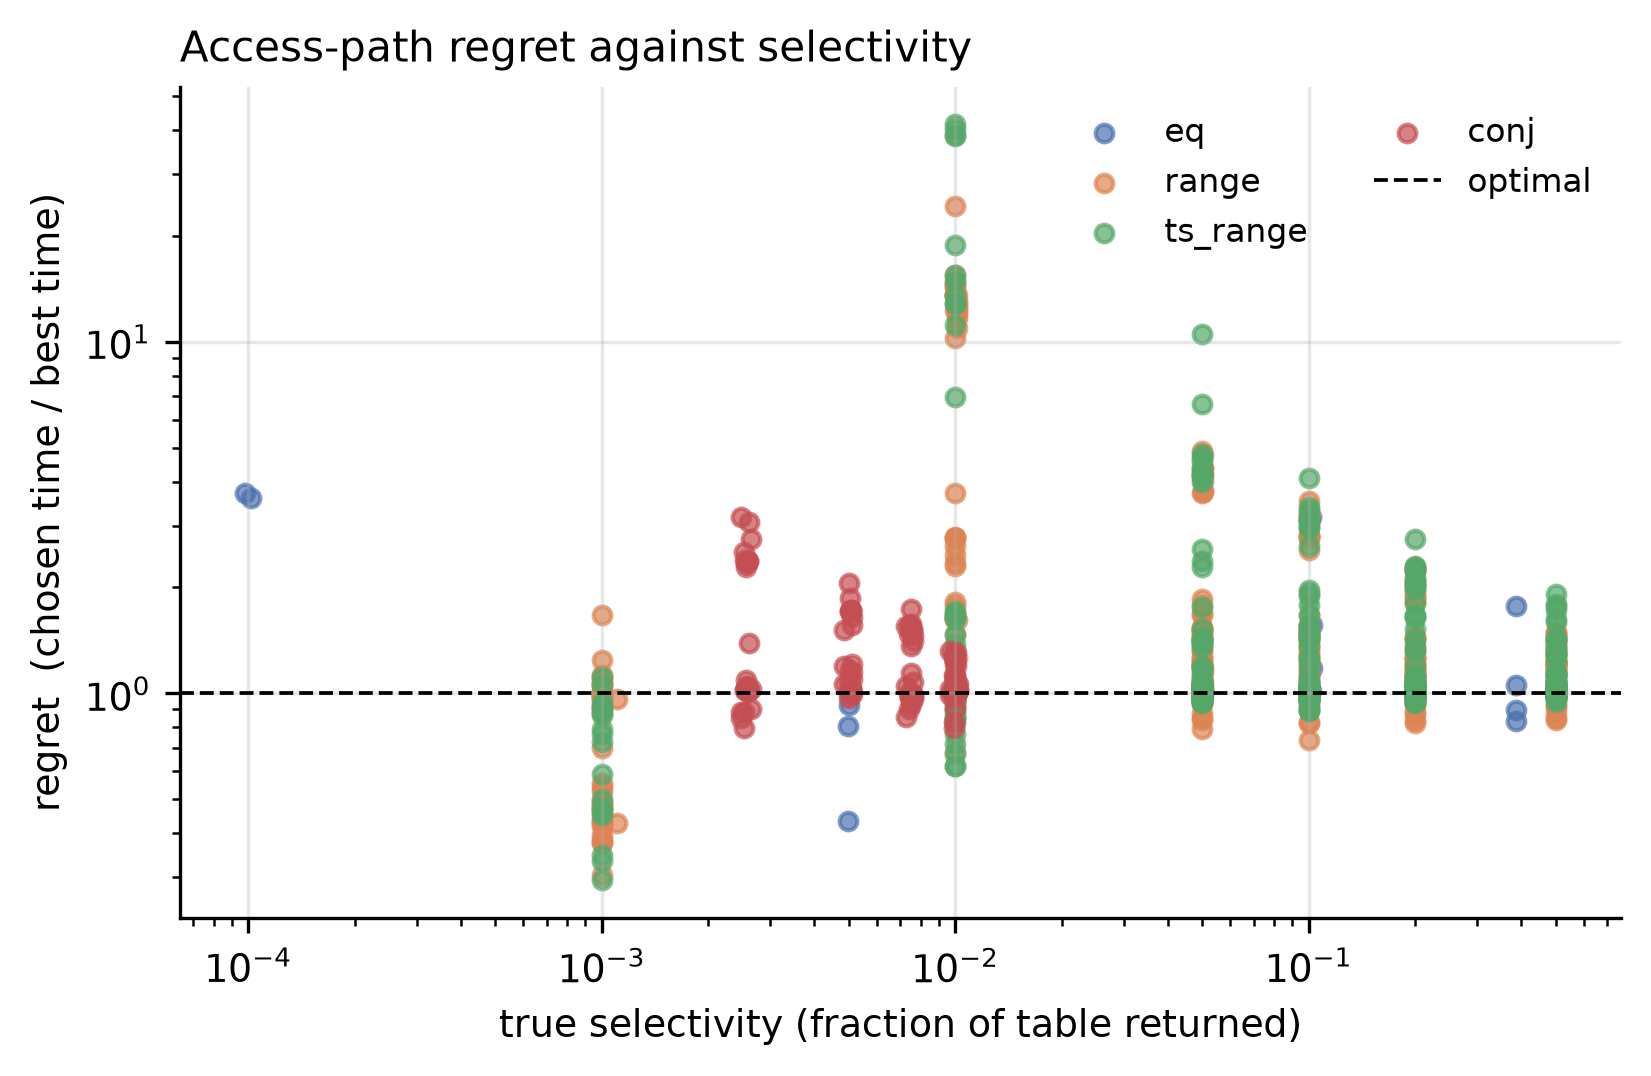
\includegraphics[width=0.68\linewidth]{figures/fig2_regret_by_selectivity.png}
\caption{Access-path regret against true selectivity, by query family.
Both axes logarithmic; the dashed line marks an optimal choice. Errors
cluster in the band where index and sequential costs cross.}
\label{fig:regret}
\end{figure}

Figure~\ref{fig:estimation} separates estimation error by its source.
Panel A shows the effect of column correlation on conjunctive
predicates, the dependent and independent variants diverging as the
dependency strengthens while the independent control stays flat, which
confirms the generator induced correlation rather than merely noise.
Panel B shows single-column predicates, where estimation is accurate
across four orders of magnitude of selectivity. The contrast localises
PostgreSQL's estimation weakness precisely: not selectivity in general,
but conjunction across correlated columns.

\begin{figure}[htbp]
\centering
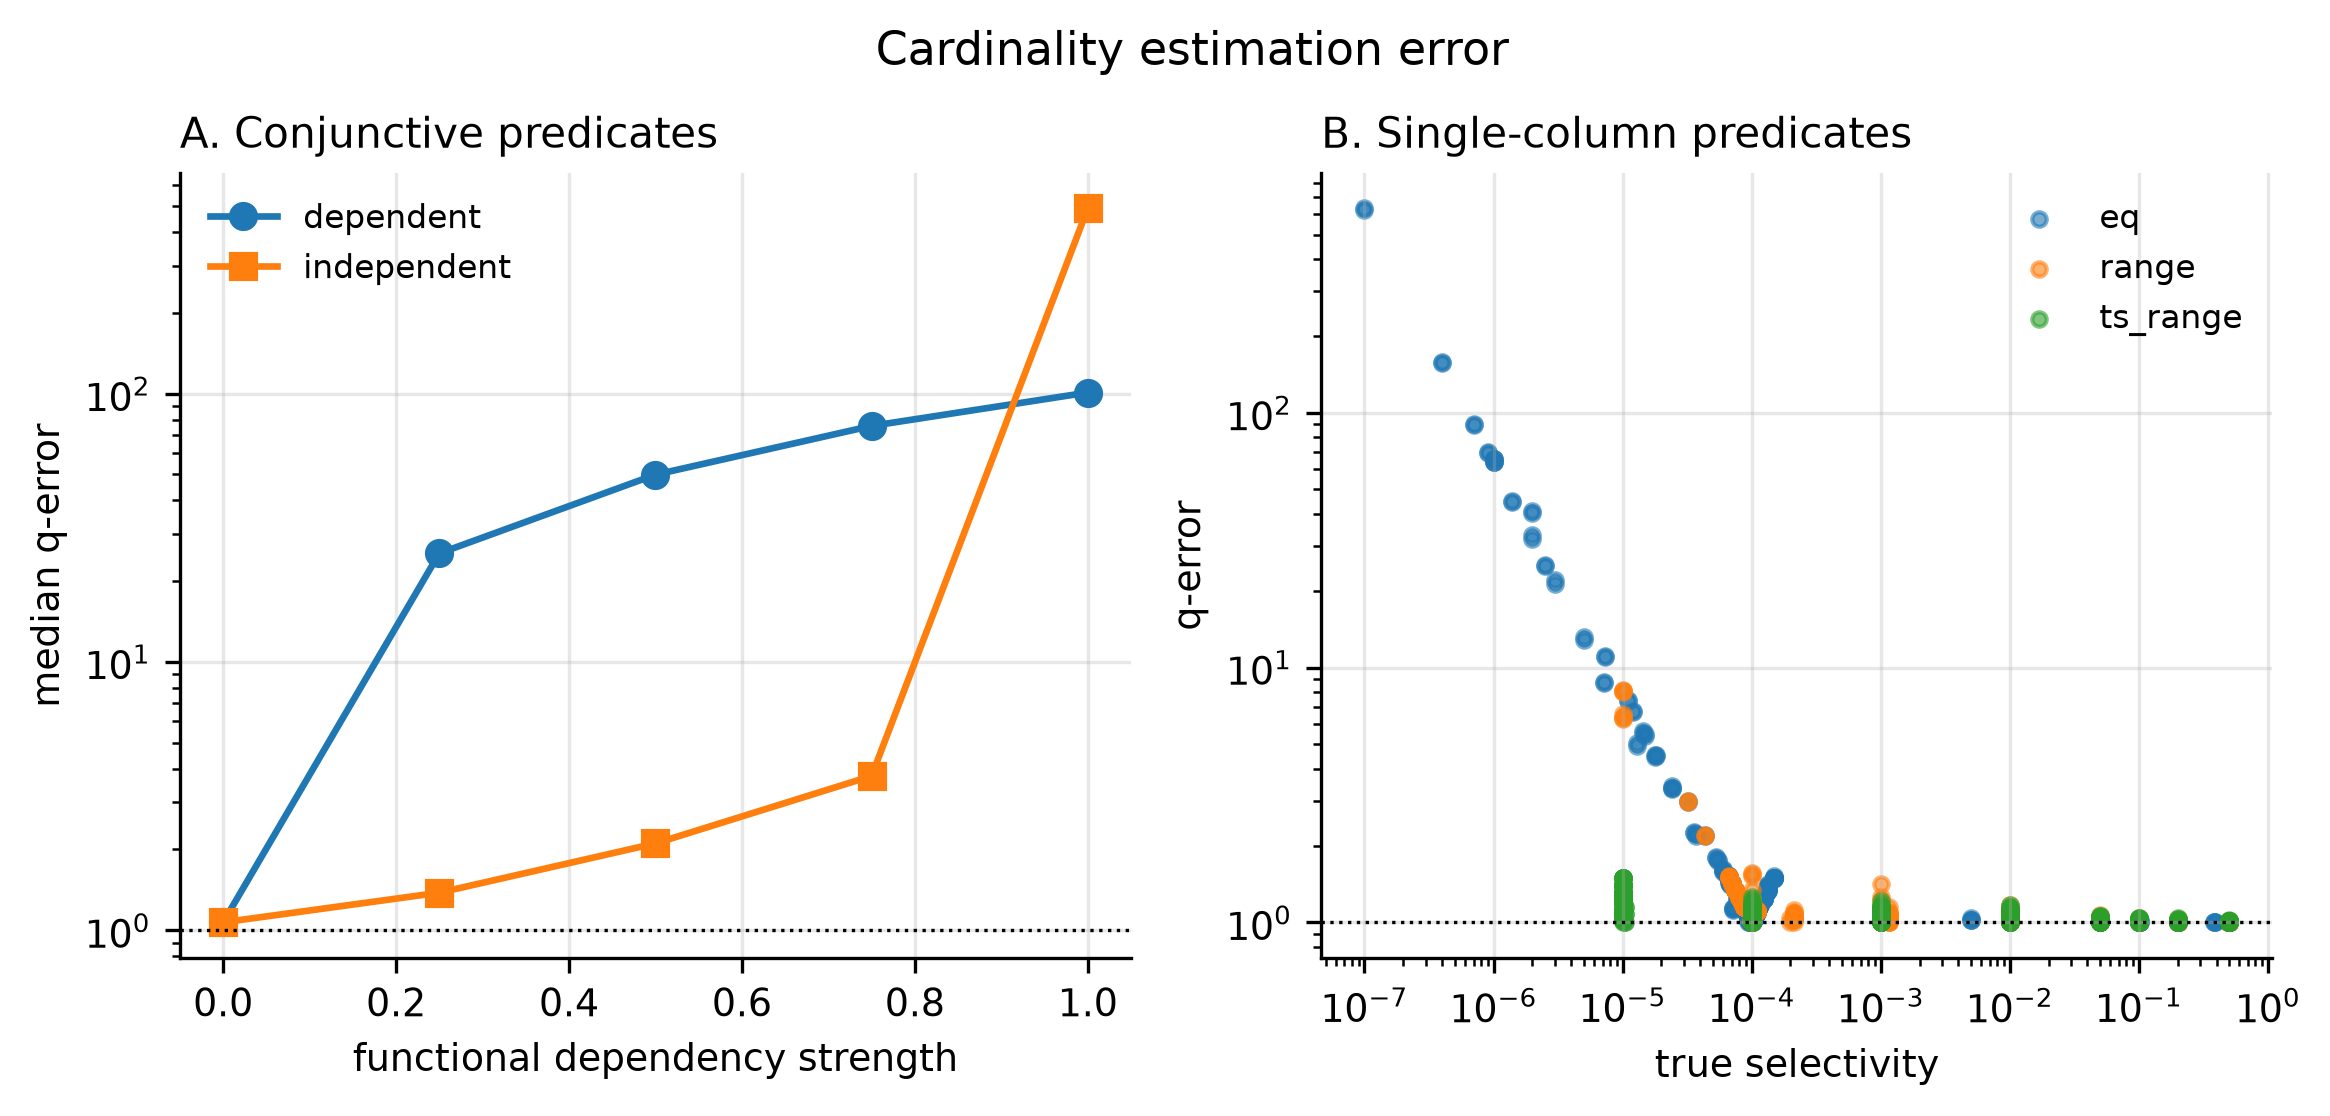
\includegraphics[width=0.95\linewidth]{figures/fig1_estimation_error.png}
\caption{Cardinality estimation error by source. Panel A, conjunctive
predicates against dependency strength, with the independent variant as
control. Panel B, single-column predicates against selectivity.}
\label{fig:estimation}
\end{figure}

Finally, Figure~\ref{fig:brincorr} shows why the BRIN result depends so
completely on physical clustering. Each index configuration is plotted
against the correlation between value order and row order. BRIN is
competitive only as that correlation approaches unity; everywhere else
it reads most of the table.

\begin{figure}[htbp]
\centering
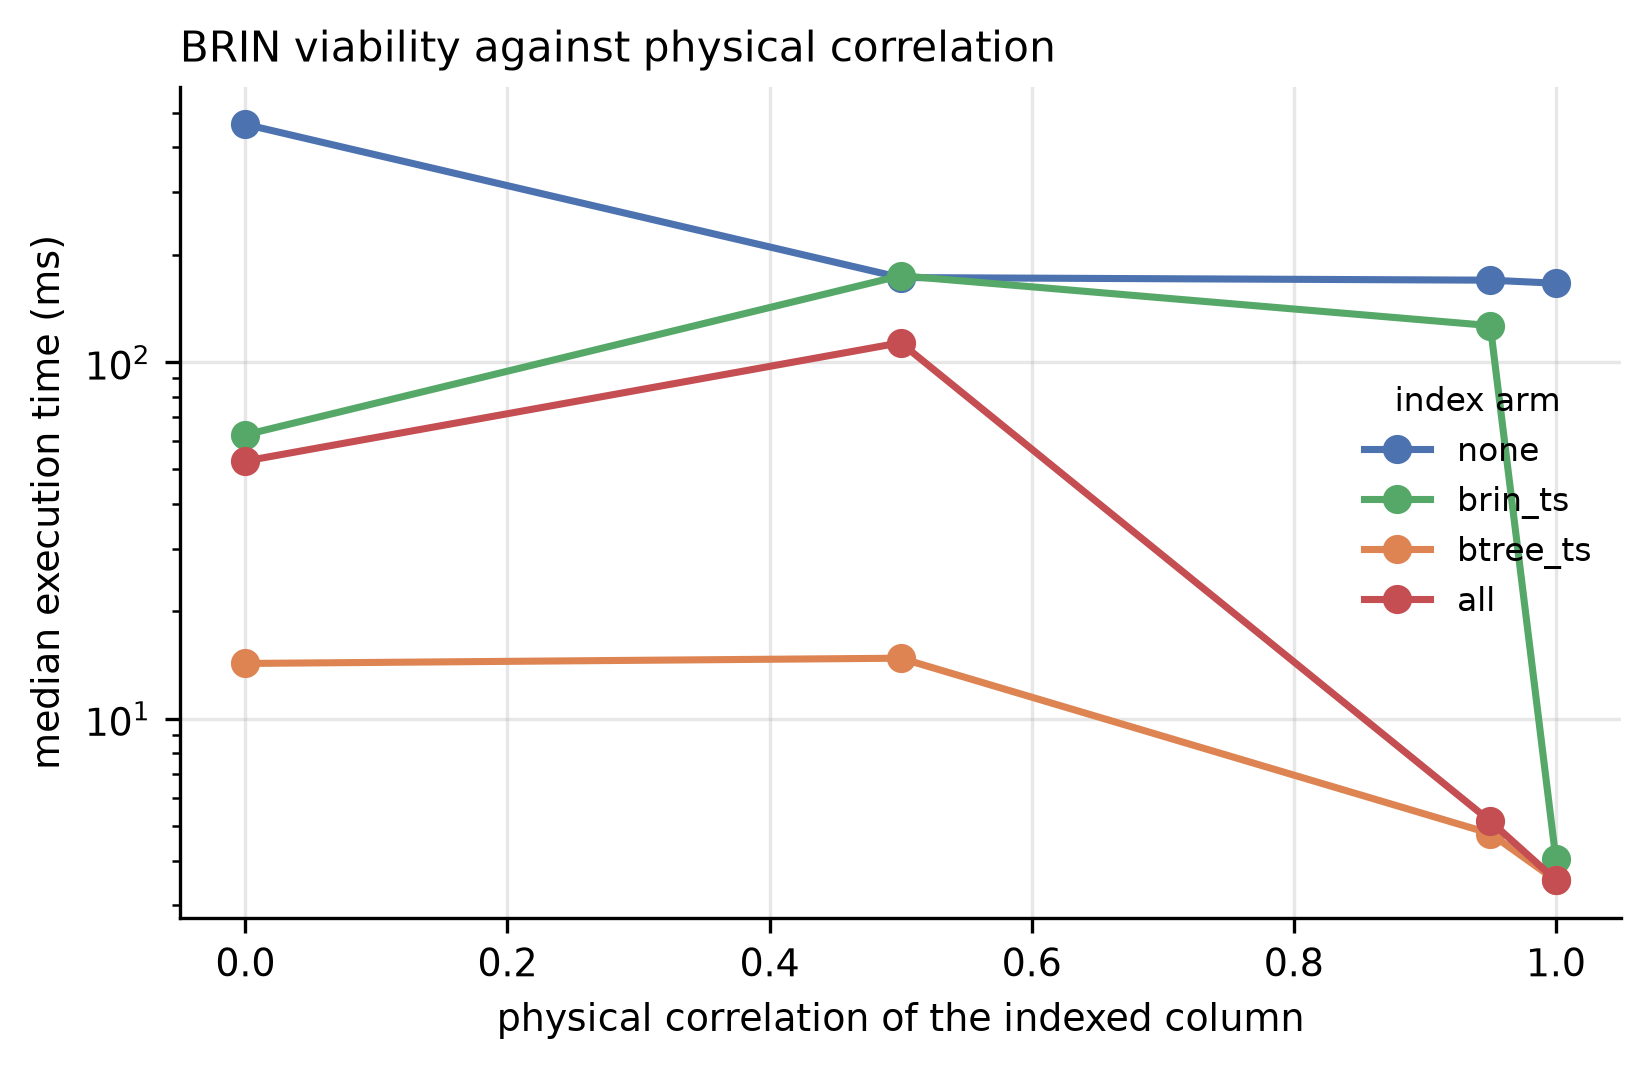
\includegraphics[width=0.66\linewidth]{figures/fig5_brin_correlation.png}
\caption{Execution time against physical correlation of the indexed
column, by index configuration. Logarithmic vertical axis.}
\label{fig:brincorr}
\end{figure}

%=====================================================================
\section{Discussion}
\label{sec:discussion}
%=====================================================================

\subsection{A common failure pattern}

The three practices fail for a shared reason: each optimises a single
quantity, while plan quality depends on several.

Extended statistics optimise \emph{estimate accuracy}. A more accurate
estimate improves the plan only if it is applied consistently wherever
the plan is priced, and Section~\ref{sec:extstats} shows it is not. The
partial correction is worse than no correction, because it makes two
candidate paths priced under different assumptions directly comparable
when they are not.

Reducing \rpc{} optimises for \emph{storage latency}. The premise is
sound: random access on flash is cheaper relative to sequential access
than the default assumes \citep{graefe2009fast}. But the same constant
governs the choice between bitmap and plain index access, so reducing
it improves one decision while degrading another, and
Section~\ref{sec:rpc} shows the second effect dominates below 1.5.

Adding a BRIN index optimises for \emph{index size and construction
cost}, on both of which BRIN genuinely excels. But index availability
also determines which paths the optimiser generates, and
Section~\ref{sec:brin} shows a cheap index can capture the bitmap path
and exclude a superior one.

In each case the advice is correct about the quantity it names and
wrong about the outcome. This generalises beyond the three specific
cases: mechanism-based tuning advice is systematically vulnerable to
this failure whenever the mechanism is real but not the only mechanism
in play. The corrective is workload-level measurement, which is exactly
what such advice typically lacks.

\subsection{Reporting boundaries}

Section~\ref{sec:boundary} carries a methodological point beyond its
specific finding. Our own two-point comparison would have supported a
conclusion the intermediate measurements refute, and the refutation was
not a matter of degree but of direction: severity increases where the
two-point reading suggests it decreases.

We suggest that empirical database studies reporting a performance
effect should, where feasible, also report the conditions under which
it ceases to hold. Without that, practitioners cannot determine
applicability, and apparent contradictions between studies measuring at
different scales cannot be distinguished from genuine disagreement.

\subsection{Recommendations for practitioners}

\begin{enumerate}
\item Do not create extended statistics reflexively. Verify that the
  \emph{plan} improved, not merely the estimate; the two are separable
  and can move in opposite directions.
\item Do not reduce \rpc{} below approximately 1.5 without workload
  measurement. The default was within 6\% of optimal here.
\item Treat a BRIN index co-located with a B-tree on the same column as
  a risk requiring measurement, with particular attention when the
  table is between one and three times \sbuf{}.
\item Do not assume hash index construction is inexpensive on skewed
  columns.
\end{enumerate}

%=====================================================================
\section{Threats to Validity}
\label{sec:threats}
%=====================================================================

\paragraph{Internal validity}
Regret is a lower bound, since the denominator is the fastest measured
configuration rather than a proven optimum. Values marginally below
$1.0$ occur because the free-choice configuration can combine indexes
in ways no single restricted configuration can, which we report rather
than clamp. The misselection threshold of $1.2$ is a judgement call;
full distributions are published so that alternatives may be applied.

\paragraph{Construct validity}
The path-elimination mechanism in Section~\ref{sec:brin} is confirmed
against the PostgreSQL~17 source, but our reading of that source is
static. We did not instrument the planner to observe the discarded path
directly, so the identification rests on the code path being the only
one consistent with the observed costs. The extended-statistics result
requires a redundant index set, a
composite index alongside both single-column indexes, which is common
in practice but not universal; where only the composite index exists
the effect cannot arise.

\paragraph{External validity}
The study covers two DBMSs on one hardware configuration, and the
MariaDB arm is measured at a single scale rather than across the seven
used for PostgreSQL, so the scale boundaries of
Section~\ref{sec:boundary} are established for PostgreSQL only. Two
systems are sufficient to show that a behaviour is not universal, as
with selection quality, and are suggestive but not conclusive when both
agree, as with the merge-plan failure: two optimisers may share an
inherited design assumption without it being necessary. A third
independently developed optimiser would strengthen that claim.
All measurements are warm-cache;
reliably evicting the operating system page cache is not portable, so
cold-storage behaviour is out of scope rather than approximated.
Because the host has 23.8\,GB of memory, the page cache retains the
data even at $10^7$ rows, so our larger scales test departure from the
\emph{buffer pool} rather than from memory, and the two cannot be
separated on this hardware. Only single-relation access paths are
considered; join ordering is deliberately excluded as a separate and
well-studied problem \citep{leis2018query}.

%=====================================================================
\section{Conclusion}
\label{sec:conclusion}
%=====================================================================

PostgreSQL~17's access-path selection is close to optimal under a
conventional index set, selecting the best available plan for 97.7\% of
the queries measured. Where it fails, cardinality misestimation is not
the cause: 98.2\% of misselected queries had accurate row estimates, in
contrast to the established result for join ordering.

That quality is an implementation property rather than a general one.
The same workload on MariaDB~10.4 misselects for 66.0\% of queries,
because it lacks the bitmap middle ground PostgreSQL uses to convert
random heap access into ordered access, falling back instead to plain
index lookups or full scans.

The failures instead trace to cost modelling and path generation, and
are triggered by three practices intended to prevent them. Extended
statistics improve estimates by up to 108$\times$ and slow queries by
up to 2.7$\times$, because the correction is not propagated to the
\texttt{BitmapAnd} node. Reducing \rpc{} on flash storage costs a
factor of 2.3, the default lying within 6\% of optimal. A co-located
BRIN index raises misselection from 2.3\% to 73.3\% and can slow
individual queries by 194$\times$.

That last effect has two boundaries rather than one. Its frequency
collapses when the heap exceeds \sbuf{}, while its worst case doubles
at that same point and subsides only when queries begin incurring
physical reads. The most severe regressions occur at two to three times
the buffer pool size, not at the smallest scale, and a two-point
comparison would have indicated the opposite.

A tuning recommendation is not correct or incorrect in isolation; it is
correct or incorrect under conditions, and those conditions are
measurable. Reporting an effect without its boundaries invites
practitioners to apply it where it does not hold, or to dismiss it
where it does.

\paragraph{Future work}
Three directions follow. The deduplication tiebreak identified in
Section~\ref{sec:brin} suggests a concrete remedy worth evaluating:
breaking ties on estimated bitmap precision, or on
\texttt{bitmap\_scan\_cost\_est()} rather than index-side cost alone,
at the price of additional planning time. Quantifying that trade-off is
a natural follow-up. Extending the MariaDB arm across the full range of
scales would establish whether the buffer-pool boundaries of
Section~\ref{sec:boundary} are likewise implementation-specific, and a
third independently developed optimiser would test whether the
merge-plan weakness is genuinely architectural or a shared inherited
assumption. Extending to hardware permitting
controlled page-cache eviction would separate buffer-pool residency
from operating-system cache residency, a distinction the present
platform cannot make.

%=====================================================================
\section*{Data availability}
All source code, raw measurements, generated figures and an executable
analysis notebook are publicly available \citep{artifact2026}. No
dataset is distributed: all data is generated from a fixed seed, so the
corpus is byte-identical on any machine. Measurement runs are resumable
at the granularity of a single execution, and each record retains all
individual repetitions rather than only the median, so variance claims
can be verified independently.

\section*{CRediT authorship contribution statement}
\textbf{Md. Imtiaj Alam Sajin:} Conceptualization, Methodology,
Software, Validation, Formal analysis, Investigation, Data curation,
Writing -- original draft, Visualization.
\textbf{Ashraf Uddin:} Supervision, Writing -- review and editing.

\section*{Declaration of competing interest}
The authors declare no competing financial interests or personal
relationships that could have influenced the work reported in this
paper.

\bibliographystyle{elsarticle-harv}
\bibliography{references}

\end{document}
